\documentclass{tufte-handout}
\usepackage[utf8]{inputenc}
\usepackage{parskip}
\usepackage{amssymb, amsthm, amsmath, fdsymbol, mathtools, cancel, extarrows} % Varios paquetes para símbolos y fuentes
\usepackage{tikz, pgfplots} % Para dibujar
\usepackage{tkz-graph, tkz-berge} % Para dibujar grafos
\usepackage[linguistics]{forest} % Para dibujar árboles
\useforestlibrary{edges}
\usepackage{algorithm2e} % Para escribir pseudocódigo
\usepackage{titling} % Para estilizar el título
\usepackage{scrextend} % Añade márgenes para hacer bloques de texto
\usepackage{enumitem} % Para enumerar sin sangría
\usepackage{graphicx, subcaption} % Para colocar figuras e imágenes
\usepackage{lastpage}
\usepackage{fancyhdr} % Para hacer encabezados y pie de página más estilizados
\usepackage{color} % Para usar colores en el texto
\usepackage{soul} % Para subrayar con colores
\usepackage{soulutf8}
\usepackage{titling} % Cambia los parámetros del título
\usepackage{booktabs} % Para hacer tablas un poco más estilizadas
\usepackage{multirow}

% Cambia el tamaño de los captions
\usepackage[font={footnotesize}]{caption}

% Establece los enviroments para teoremas, ejemplos, definiciones, etc
\newtheorem{teo}{Teorema}
\newtheorem{cor}[teo]{Corolario}
\newtheorem{lem}[teo]{Lema}
\newtheorem{pro}[teo]{Proposición}
\newtheorem{pre}{Pregunta}

\theoremstyle{definition}
\newtheorem{defn}{Definición}
\newtheorem{ejem}{Ejemplo}
\newtheorem{ejer}{Ejercicio}
\newtheorem{notn}{Notación}
\newtheorem{nota}{Nota}
\newtheorem{prob}{Problema}

% Comandos para símbolos
\newcommand{\Nastk}{\mathbb{N}^*}
\newcommand{\N}{\mathbb{N}}
\newcommand{\Z}{\mathbb{Z}}
\newcommand{\C}{\mathbb{C}}
\newcommand{\R}{\mathbb{R}}
\newcommand{\prop}{\mathcal{P}}
\newcommand{\con}{\sim_{c}}
\newcommand{\ent}{\operatorname{entrada}}
\newcommand{\sal}{\operatorname{salida}}
\newcommand{\val}{\operatorname{val}}
\newcommand{\sumtoinfty}[2]{\sum_{#1}^{\infty} #2}

% Cambia el nombre de varios comandos
\renewcommand{\contentsname}{Contenido}
\renewcommand*{\proofname}{Demostración}
\renewcommand{\figurename}{Fig.}

% Establece las notas de margen
\newcommand{\marginfootnote}[1]{\footnotemark\footnotetext{#1}}

% Establecemos cómo será el encabezado y el pie de página
\fancyhf{}
\pagestyle{fancy}
\fancyhf{}
\fancyhead[L]{MA-4411}
\fancyhead[C]{Eduardo José Gavazut Pinto}
\fancyhead[R]{13-10524}
\fancyfoot[L]{Sección 1}
\fancyfoot[R]{Profesor: Jesús Nieto}
\fancyfoot[C]{\thepage\ de \pageref{LastPage}}
\renewcommand{\headrulewidth}{2pt} 
\renewcommand{\footrulewidth}{2pt}

% Establece los entornos para los bloques de pseudocódigo
\RestyleAlgo{ruled}
\newenvironment{algoritmo}[1][htb]
  {\renewcommand{\algorithmcfname}{Algoritmo}% Update algorithm name
   \begin{algorithm}[#1]%
  }{\end{algorithm}}

% Establece el entorno para hacer diagramas de Ferrers
\newenvironment{ferrers}[1][4em]
 {%
  \leavevmode
  \hbox\bgroup
    \def\\{\unskip\cr\noalign{\hskip#1}}%
    \valign\bgroup&##\cr
 }
 {%
  \unskip\crcr\egroup
  \egroup
 }

\newcommand{\row}[1]{%
  \hbox{$\activatem\romannumeral\number\number#1 000 \unskip$}\vskip 0.5em plus 3em
}
\newcommand{\activatem}{%
  \begingroup\lccode`~=`m \lowercase{\endgroup\def~}{\bullet\hskip1em}%
  \mathcode`m="8000
}

% Define la geometría del margen
\geometry{
	left=13mm, % left margin
	textwidth=130mm, % main text block
	marginparsep=8mm, % gutter between main text block and margin notes
	marginparwidth=55mm % width of margin notes
}

% Permite agregar etiquetas a los niveles de un árbol
\forestset{%
  label tree/.style={
    for tree={tier/.option=level},
    level label/.style={
      before typesetting nodes={
        for nodewalk={current,tempcounta/.option=level,group={root,tree breadth-first},ancestors}{if={>OR={level}{tempcounta}}{before drawing tree={label me=##1}}{}},
      }
    },
    before drawing tree={
      tikz+={\coordinate (a) at (current bounding box.east);},
    },
  },
  label me/.style={tikz+={\node [anchor=base north] at (.parent |- a) {#1};}},
}

% Establece el subrayado de color rojo
\definecolor{ferrari}{rgb}{1,0.17,0}
\setulcolor{ferrari}

% Reduce el espacio entre el título y el header
\setlength{\droptitle}{-5.5em}
\renewcommand\maketitlehookc{\vspace{-3ex}}

% Define el espaciado entre párrafos
\setlength{\parskip}{1.5em}

% Definimos nuestro título
\pretitle{\begin{flushleft}\LARGE\sffamily}
\title{
Notas de Combinatoria, Abril-Julio 2022 \\
Universidad Simón Bolívar
}
\posttitle{\par\end{flushleft}\vskip 0.5em}
\preauthor{\begin{flushleft}\large\scshape}
\author{
Eduardo Gavazut \\
Carnet: 13-10524}
\postauthor{\par\end{flushleft}}
\predate{\begin{flushleft}\large\scshape}
\date{Abril-Julio 2022}
\postdate{\par\end{flushleft}}

% Aquí empieza el documento
\begin{document}

\maketitle
\thispagestyle{fancy}

\tableofcontents
\break
\section{Repaso de Derivada}
\stepcounter{sec}

Haremos primero un repaso de la derivada, concepto fundamental del cálculo diferencial. Trataremos ante todo las derivadas de funciones de una variable real, más especialmente de funciones reales definidas en intervalos de $\R$.

\begin{defn}
    Sea $f$ una función real definida en un intervalo abierto $(a, b)$, y supongamos que $c \in \R$ es un punto tal que $c \in (a, b)$. Diremos que $f$ es diferenciable en $c$ siempre que el límite
    
    \[
    \lim_{x \to c} \frac{f(x) - f(c)}{x-c}
    \]
    
    \noindent exista. Este límite, denotado por $f'(c)$ se llama \ul{derivada} de $f$ en $c$.
\end{defn}

Esta forma de calcular límites define una nueva función $f'$ cuyo dominio está formado por aquellos puntos de $(a, b)$ en los que $f$ es diferenciable. La función $f'$ se llama la \ul{primera derivada} de $f$. De forma análoga, la $n$-ésima derivada de $f$ se designa por $f^{(n)}$, y es la primera derivada de $f^{(n-1)}$, para $n = 2, 3, \dots$

\begin{teo}[Teorema del Valor Medio (T.V.M)]\label{teo:1.1.1}
    Si $f$ está definida en un intervalo $(a, b)$ y es diferenciable en un punto $c$ de $(a, b)$, entonces existe una función $f^*$ (que depende de $f$ y $c$) continua en $c$ y que satisface la ecuación
    
    \begin{equation}\label{eq:1.1.1}
        f(x) - f(c) = (x-c)f^*(x)
    \end{equation}
    
    \noindent para todo $x$ de $(a, b)$, con $f^*(c) = f'(c)$. Recíprocamente, si existe una función $f^*$ continua en $c$, que satisface la ecuación anterior, entonces $f$ es diferenciable en $c$ y $f'(c) = f^*(c)$.
\end{teo}

\begin{proof}
    Si $f$ es diferenciable en $c$, entonces $f'(c)$ existe. Definamos ahora $f^*$  en $(a, b)$ como sigue:
    
    \[
    f^*(x) = 
    \begin{cases}
        \dfrac{f(x) - f(c)}{x-c} & \text{si $x \neq c$} \\
        f'(c) & \text{e.o.c}
    \end{cases}
    \]
    
    Entonces $f^*$ es continua en $c$ y \ref{eq:1.1.1} se verifica para todo $x$ de $(a, b)$.
    
    Recíprocamente, si \ref{eq:1.1.1} se verifica para alguna función $f^*$ continua en $c$, entonces dividiento por $x-c$ y haciendo tender $x$ a $c$, vemos que $f'(c)$ existe y es igual a $f^*(c)$.
\end{proof}

Como consecuencia directa de este teorema tenemos:

\begin{teo}
    Si $f$ es diferenciable en $c$, entonces $f$ es continua en $c$.
\end{teo}

\begin{proof}
    Se demostró en el teorema anterior. Basta con hacer $x \to c$.
\end{proof}

Ahora describiremos las fórmulas para diferenciar la suma, la resta, el producto, y el cociente de dos funciones:

\begin{teo}
    Supongamos que $f$ y $g$ están definidas en $(a, b)$ y son diferenciables en $c$. Entonces $f+g$, $f-g$ y $f \cdot g$ son también diferenciables en $c$. Esto es así para $f / g$ si $g(c) \neq 0$. Las derivadas de $c$ están dadas por
    
    \begin{enumerate}
        \item $(f \pm g)'(c) = f'(c) \pm g'(c)$.
        \item $(f \cdot g)'(c) = f(c)g'(c) + f'(c)g(c)$.
        \item $(f/g)'(c) = \dfrac{g(c)f'(c) - f(c)g'(c)}{g(c)^2}$, si $g(c) \neq 0$.
    \end{enumerate}
\end{teo}

Y finalmente, describiremos la regla de la cadena:

\begin{teo}[Regla de la cadena]
    Sea $f$ definida en un intervalo abierto $S$ y sea $g$ definida en $f(S)$ y consideremos la función compuesta $g \circ f$ definida en $S$ por medio de la ecuación
    
    \[
    (g \circ f)(x) = g(f(x))
    \]
    
    Supongamos que existe un punto $c$ de $S$ tal que $f(c)$ sea un punto interior de $f(S)$. Si $f$ es diferenciable en $c$ y $g$ es diferenciable en $f(c)$, entonces $g \circ f$ es diferenciable en $c$ y se tiene que
    
    \[
    (g \circ f)'(c) = f'[f(c)]f'(c)
    \]
\end{teo}

\begin{proof}
    Usando el teorema \ref{teo:1.1.1}, tenemos que
    
    \[
    f(x) - f(c) = (x-c)f^*(x)
    \]
    
    \noindent para todo $x$ de $S$. Donde $f^*$ es continua en $c$ y $f^*(c) = f'(c)$. En particular,
    
    \[
    g(y) - g[f(c)] = [y - g(c)]g^*(y)
    \]
    
    \noindent para todo $y$ de un cierto subintervalo abierto $T$ de $f(S)$ que contenga a $f(c)$. Aquí, $g^*$ es continua en $f(c)$ y $g^*(f(c)) = g'[f(c)]$.
    
    Ahora pasemos a elegir un $x \in S$ tal que $y = f(x) \in T$. Entonces
    
    \begin{equation}\label{eq:1.1.2}
        g[f(x)] - g[f(c)] = [f(x) - g(c)]g^*[f(x)] = (x-c)f^*(x)g^*[f(x)]
    \end{equation}
    
    Por el teorema de continuidad de las funciones compuestas\marginfootnote{Si la función $g$ es continua en $a$ y la función $f$ es continua en $g(a)$, entonces la función compuesta $f \circ g$ es continua en $a$.},
    
    \[
    g^*[f(x)] \rightarrow g^*[f(c)] = g'[f(c)] \quad \text{cuando $x \rightarrow c$}
    \]
    
    Por lo que si dividimos \ref{eq:1.1.2} por $x-c$, y hacemos $x \rightarrow c$ obtenemos
    
    \[
    \lim_{x \to c} \frac{f[f(x)] - g[f(c)]}{x-c} = g'[f(c)]f'(c)
    \]
    
    \noindent como queríamos.
\end{proof}

\section{Funciones Diferenciables}
\addtocounter{sec}{1}

Esta parte del curso se centrará en el estudio de las funciones diferenciables, sus propiedades y aplicaciones. Además estudiaremos dos teoremas centrales cuyas demostraciones no son triviales: El teorema de la función implícita y el teorema de la función inversa.

\subsection{Campos escalares y vectoriales}
\stepcounter{subsec}

Empezamos esta primera parte estudiando la noción de diferenciabilidad para funciones escalares definidas de $\R^n$ en $\R$ (a las cuales llamaremos campos escalares) y para funciones vectoriales definidas de $\R^n$ en $\R^m$ (que llamaremos campos vectoriales), con $n,m \in \N$.

Para ello introduciremos primero las definiciones de derivada direccional, derivada parcial, operador gradiente y el jacobiano de una función.

\begin{defn}
    Sean $A \subseteq \R^n$ abierto, conexo y convexo y $f: A \rightarrow \R$ tal que $f$ es continua. Entonces
    
    \[
    \delta_i f(x_0) = \frac{\delta f}{\delta x_i}(x_0)
    \]
    
    \noindent son las \ul{derivadas parciales} de $f$ respecto a $i$-ésima variable son las funciones con valores reales, y vienen dadas por
    
    \[
    \delta_i f(x_0) = \lim_{h \to 0} \frac{f(x_0 + h \cdot e_i) - f(x_0)}{h}
    \]
    
    \noindent donde $h \in \R$, y $e_i = (0, 0, \dots, 1, \dots, 0)$, con el $1$ en la $i$-ésima coordenada.
\end{defn}

\begin{teo}
    Sean $A \subseteq \R^n$ abierto, conexo y convexo, con $f: A \rightarrow \R$ de clase $C^2(A)$\marginfootnote{Es decir, que $f$, $\delta_if, \delta^2_{ij}f$ para todo $i,j=1, \dots, n$ existen en cada punto de $A$ y además son continuas.}. Entonces
    
    \[
    \delta_k\delta_if = \delta_i\delta_kf
    \]
\end{teo}

\begin{proof}
    Consideremos primero para el caso $n = 2$: Queremos verificar que
    
    \[
    \delta_1\delta_2f = \delta_2\delta_1f
    \]
    
    Sean $(x_1, x_2) \in A$ y $h_1, h_2 \in \R$. Definamos la función $g: (x,y) \rightarrow \R$ (donde $(x,y)$ es un conjunto abierto perteneciente a $A$) de la siguiente manera
    
    \[
    g(x_1) = f(x_1, x_2 + h_2) - f(x_1, x_2)
    \]
    
    Como $f$ es continua, entonces $g$ es continua también. Además $g$ es derivable porque tenemos como hipótesis que es $f$ derivable con respecto a cada una de las variables. En consecuencia, $g$ es derivable en el punto $x_1$. Consideremos $g$ sobre el intervalo $[x_1, x_1 + h_1]$, aplicando el \TVM, existe $S_1 \in (x_1, x_1 + h_1)$ tal que satisface
    
    \[
    g'(S_1) = \frac{g(x_1 + h_1) - g(x_1)}{h_1}
    \]
    
    Por lo tanto, tenemos que
    
    \begin{align*}
        f(x_1 + h_1, &x_2 + h_2) - f(x_1 + h_1, x_2) - f(x_1, x_2 + h_2) + f(x_1, x_2) \\
            &= g(x_1 + h_1) - g(x_1) = h_1 \cdot g'(S_1) \\
            &= h_1 \left[ \delta_1 f(S_1, x_2 + h_2) - \delta_1 f(S_1, x_2) \right]
    \end{align*}
    
    Como la función $f$ es de clase $C^2$, nuevamente podemos aplicar el \TVM, y nos queda que
    
    \begin{align}\label{eq:1.2.1}
        h_1 \big[ \delta_1 f(&S_1, x_2 + h_2) - \delta_1 f(S_1, x_2) \big] \nonumber \\
            &= h_1h_2 \delta_2\delta_1 f(S_1, S_2)
    \end{align}
    
    \noindent con $S_2 \in (x_2, x_2 + h_2)$.
    
    Nuevamente, ahora si consideramos $\hat{g}(x_2) = f(x_1 + h_1, x_2) - f(x_1, x_2)$, podemos repetir el mismo argumento y podemos concluir que existen $t_1 \in (x_1, x_1 + h_1)$ y $t_2 \in (x_2, x_2 + h_2)$ tales que
    
    \begin{align}\label{eq:1.2.2}
        f(x_1 + h_1, &x_2 + h_2) - f(x_1 + h_1, x_2) - f(x_1, x_2 + h_2) + f(x_1, x_2) \nonumber \\
            &= h_1h_2 \delta_1\delta_2 f(t_1, t_2)
    \end{align}
    
    Al hacer $(h_1, h_2) \to (0, 0)$, como las derivadas parciales existen (tanto las de primer como segundo grado), podemos concluir por \ref{eq:1.2.1} y \ref{eq:1.2.2} que
    
    \[
    \delta_1\delta_2 f(x_1, x_2) = \delta_2\delta_1 f(x_1, x_2)
    \]
    
    Y así queda demostrado el teorema para $n=2$. Para $n>2$ el procedimiento es el mismo, pero hay que tener más cuidado con la notación:
    
    Sean el vector $x_0 = (x_0^1, x_0^2, \dots, x_0^n) \in A$, y $h_i, h_j \in \R$ con $i \neq j$, $(i < j)$. Definamos nuevamente una función auxiliar para $x, y \in \R$
    
    \[
    \Phi(x,y) = f(x_0^1, x_0^2, \dots, x, \dots, y, \dots, x_0^n)
    \]
    
    \noindent donde $x$ está en la $i$-ésima coordenada e $y$ está en la $j$-ésima coordenada. Esto para todo $(x, y) \in U$, donde $U$ es un abierto que contiene a $(x_0^i, x_0^j)$. Sea ahora
    
    \[
    g(x_0^i) = \Phi(x_0^i, x_0^j + h_j) - \Phi(x_0^i, x_0^j)
    \]
    
    Como $f$ es de clase $C^2(A)$, entonces $\Phi$ y $g$ son continuas y derivables en $x_0^i$ y $(x_0^i, x_0^i + h_i)$ respectivamente. Entonces podemos usar el \TVM, sobre $g$ y el intervalo $[x_0^i, x_0^i + h_i]$, y existe $S_i \in (x_0^i, x_0^i + h_i)$ tal que
    
    \[
    g(x_0^i + h_i) - g(x_0^i) = h_ig'(S_i)
    \]
    
    Luego,
    
    \begin{align*}
        \Phi(x_0^i + h_i, &x_0^j + h_j) - \Phi(x_0^i + h_0^i, x_0^j) - \Phi(x_0^i, x_0^j + h_0^j) + \Phi(x_0^i, x_0^j) \\
            &= g(x_0^i + h_i) - g(x_0^i) = h_i \cdot g'(S_i) \\
            &= h_i \left[ \delta_i \Phi(S_i, x_0^j + h_j) - \delta_i \Phi(S_i, x_0^j) \right]
    \end{align*}
    
    Como la función $f$ es de clase $C^2$, nuevamente podemos aplicar el \TVM, y nos queda que
    
    \begin{align}\label{eq:1.2.3}
        h_i \left[ \delta_i \Phi(&S_i, x_0^j + h_j) - \delta_i \Phi(S_i, x_0^j) \right] \nonumber \\
            &= h_ih_j \delta_j\delta_i \Phi(S_i, S_j)
    \end{align}
    
    Nuevamente, ahora si consideramos $\hat{g}(x_0^j) = \Phi(x_0^i + h_i, x_0^j) - \Phi(x_0^i, x_0^j)$, podemos repetir el mismo argumento y podemos concluir que existen $t_1 \in (x_0^i, x_0^i + h_i)$ y $t_2 \in (x_0^j, x_0^j + h_j)$ tales que
    
    \begin{align}\label{eq:1.2.4}
        \Phi(x_0^i + h_i, &x_0^j + h_j) - \Phi(x_0^i + h_0^i, x_0^j) - \Phi(x_0^i, x_0^j + h_0^j) + \Phi(x_0^i, x_0^j) \nonumber \\
            &= h_ih_j \delta_i\delta_j \Phi(t_i, t_j)
    \end{align}
    
    De esta manera, de \ref{eq:1.2.3} y \ref{eq:1.2.4} tenemos que
    
    \begin{gather*}
        h_ih_j \delta_j\delta_i f(x_0^1, \dots, S_i, \dots, S_j, \dots, x_0^n) \\
        = h_ih_j \delta_i\delta_j f(x_0^1, \dots, t_i, \dots, t_j, \dots, x_0^n)
    \end{gather*}
    
    Al hacer $(h_i, h_j) \to (0, 0)$, como las derivadas parciales existen (tanto las de primer como segundo grado), podemos concluir que
    
    \[
    \delta_i\delta_j f(x_0) = \delta_j\delta_i f(x_0)
    \]
    
    Y queda finalizada la demostración del teorema.
\end{proof}

\begin{defn}
    Sea $A \subseteq \R^n$ (con $n \in \N$) abierto, conexo y convexo. Sea también una función $f: A \rightarrow \R$ (es decir, a valores escalares) continua. El \ul{gradiente} de dicha función $f$ para cada punto $x \in A$, viene dado por
    
    \[
    \grad f(x) = \left(\delta_1 f(x), \delta_2 f(x), \dots, \delta_n f(x)\right)
    \]
\end{defn}

Como se puede observar, el gradiente de $f$, $\grad f$ es un campo vectorial que está definido en $\R^n \rightarrow \R^n$

\begin{defn}
    Sean $A \subseteq \R^n$ (con $n \in \N$) abierto, conexo y convexo, una función $f: A \rightarrow \R$ continua, y $u \in A$ un vector fijo y arbitrario. Consideremos ahora
    
    \[
    \delta_u f(x_0) = \lim_{h \to 0} \frac{f(x_0 + hu) - f(x_0)}{h}
    \]
    
    \noindent con $h \in \R$. Esta es la \ul{derivada direccional} de $f$.
\end{defn}

En el caso particular en que $u = e_i$, con $i = 1, \dots, n$, tenemos que $\delta_u f(x_0)$ es la derivada parcial.

\begin{prop}
    Como resultado de la linealidad de la derivada\marginfootnote{Esto se revisa de forma exhaustiva en las secciones 4.8 y 4.9 de Cálculo Tomo II de Tom Apostol}, tenemos que
    
    \[
    \delta_u f(x_0) = u \cdot \grad f(x_0)
    \]
    
    También tenemos que
    
    \[
    \delta_u f(x_0) = \normaeuc{u} \normaeuc{\grad f(x_0)} \cos \alpha
    \]
    
    Cuando el ángulo vale $0$ o $\pi$, entonces $u$ es paralelo al gradiente de $f$ en $x_0$.
    
    En general, el gradiente apunta a la dirección de mayor declive con respecto a la curva de nivel de la superficie generada por $f$. Y en esa dirección de mayor declive, siempre podremos considerar un vector $u$ normalizado, y nos queda
    
    \[
    \delta_u f(x_0) = \normaeuc{\grad f(x_0)}
    \]
\end{prop}

\begin{defn}
    Sea $F: \R^n \rightarrow \R^k$ y supongamos que $F = (f_1, \dots, f_k)$, donde cada $f_i(x) = f_i(x_1, \dots, x_n)$ para $i = 1, \dots, k$. El \ul{jacobiano} está definido como
    
    \[
    JF(x_0) =
    \begin{pmatrix}
        \delta_1 f_1(x_0) & \dots & \delta_n f_1(x_0) \\
        \vdots & & \vdots \\
        \delta_1 f_k(x_0) & \dots & \delta_n f_k(x_0)
    \end{pmatrix}
    \]
\end{defn}

\begin{nota}
    La letra $D$ se utilizará para denotar el jacobiano, la derivada o el gradiente, dependiendo del contexto.
\end{nota}

\begin{ejem}
    Supongamos que tenemos $F: \R^2 \rightarrow \R^2$, donde
    
    \[
    F(x, y) = \left( y^2 + x^3, e^{x+y} \right)
    \]
    
    Entonces tendremos que
    
    \[
    JF(x,y) =
    \begin{pmatrix}
        3x^2    & 2y \\
        e^{x+y} & e^{x+y}
    \end{pmatrix}
    \]
    
    En particular,
    
    \[
    JF(1,1) =
    \begin{pmatrix}
        3   & 2 \\
        e^2 & e^2
    \end{pmatrix}
    \]
\end{ejem}

\begin{pre}
    La pregunta que queremos contestar a lo largo del curso es la siguiente: ¿Dada $F: \R^n \rightarrow \R^n$, existe $f: \R^n \rightarrow \R$ tal que $F = \grad f$?
    
    Si la respuesta es afirmativa, tendremos que $F$ es un \textbf{campo conservativo}.
\end{pre}

\subsection{Diferenciabilidad}
\stepcounter{subsec}

\begin{defn}
    Sea $A \subseteq \R^k$ abierto, conexo y convexo. Sea también $f: A \rightarrow \R^n$ continua. Diremos entonces que $f$ es \ul{diferenciable} en $x_0 \in A$ si $\delta_i f$ (con $i = 1, \dots, n$) existen en el punto $x_0$ y 
    
    \[
    \lim_{x \to x_0} \frac{\normaeuc{f(x) - f(x_0) - Jf(x_0)(x - x_0)}}{\normaeuc{x - x_0}} = 0 \quad \footnotemark
    \]\footnotetext{Obsérvese que si $k=1$, entonces $\normaeuc{f} = |f|$ y $Jf(x_0)$ es el gradiente de $f$ en $x_0$.}
\end{defn}

\begin{teo}
    Sea $f: A \rightarrow \R^k$ diferenciable en $x_0$ entonces $f$ es continua en $x_0$. Más aún, $\exists M > 0$ tal que
    
    \[
    \normaeuc{f(x) - f(x_0)} \leq M \normaeuc{x - x_0}
    \]
    
    \noindent si $\normaeuc{x - x_0} < \delta$ para algún $\delta < 0$.
\end{teo}

\begin{proof}
    En primer lugar, como $f$ es diferenciable tenemos que
    
    \[
    \lim_{x \to x_0} \frac{\normaeuc{f(x) - f(x_0) - Jf(x_0)(x - x_0)}}{\normaeuc{x - x_0}} = 0
    \]
    
    Por definición en términos de $\epsilon - \delta$, dado $\epsilon > 0$, $\exists \delta > 0$ tal que si $\normaeuc{x-x_0} < \delta$,
    
    \[
    \frac{\normaeuc{f(x) - f(x_0) - Jf(x_0)(x - x_0)}}{\normaeuc{x - x_0}} < \epsilon
    \]
    
    En lo particular sea $\epsilon = 1$ y fijamos $\delta = \delta_1$. Ahora podemos decir lo siguiente: Si $\normaeuc{x - x_0} < \delta_1$ entonces por desigualdad triangular,
    
    \begin{align*}
        \normaeuc{f(x) - f(x_0)} &\leq \normaeuc{f(x) - f(x_0) - Jf(x_0)(x-x_0)} + \normaeuc{Jf(x_0)(x-x_0)}\\
            & < \normaeuc{x - x_0} + \normaeuc{Jf(x_0)(x-x_0)}
    \end{align*}
    
    Ahora, toca acotar el factor $\normaeuc{Jf(x_0)(x-x_0)}$. Por definición, este jacobiano es
    
    \[
    Jf(x_0)(x-x_0) =
    \begin{pmatrix}
        \delta_1 f_1 (x_0) & \dots & \delta_n f_1 (x_0) \\
        \vdots             & \dots & \vdots             \\
        \delta_1 f_k (x_0) & \dots & \delta_n f_k (x_0)
    \end{pmatrix}
    \begin{pmatrix}
        x_1-x_0^1 \\
        \vdots    \\
        x_n-x_0^n
    \end{pmatrix}
    \]
    
    Al realizar este producto de matrices, el resultado es el siguiente vector
    
    \[
    Jf(x_0)(x-x_0) =
    \begin{pmatrix}
        \sum_{j=1}^n \delta_j f_1 (x_0) (x_j - x_0^j) \\
        \vdots \\
        \sum_{j=1}^n \delta_j f_k (x_0) (x_j - x_0^j)
    \end{pmatrix}
    \]
    
    Y tomando la norma,
    
    \[
    \normaeuc{Jf(x_0)(x-x_0)} \leq M_1\normaeuc{x-x_0}
    \]
    
    \noindent donde $\displaystyle M_1 = \left( \sum_{v = 1}^k \left( \sum_{j=1}^n \delta_j f_v(x_0) \right)^2 \right)^{1/2}$.
    
    Luego,
    
    \[
    \normaeuc{f(x) - f(x_0)} \leq (M_1 + 1)\normaeuc{x - x_0}
    \]
    
    Sea $\delta = \min(\delta_1, \epsilon / M_1 + 1)$ entonces tenemos que si $\normaeuc{x - x_0} < \delta$, podemos concluir que
    
    \[
    \normaeuc{f(x) - f(x_0)} < \varepsilon(M_1 + 1)\normaeuc{x - x_0} < \varepsilon
    \]
    
    Luego $\lim_{x \to x_0} f(x) = f(x_0)$, por lo tanto $f$ es continua. De esta forma, queda demostrado que toda función diferenciable es continua.
\end{proof}
\subsection{Eficiencia de un algoritmo}

Con lo anterior, tenemos claro que una tarea se puede llevar a cabo mediante distintos algoritmos, entonces ¿cuál es el mejor?. Podemos asignarle una \textbf{medida} o un \textbf{tamaño} a un \textbf{caso} (o instancia). Y esto es subjetivo. Por ejemplo, para calcular la suma de dos números naturales $a$ y $b$ podemos asignar como medida del caso la cantidad de dígitos del máximo entre $a$ y $b$. Luego analizamos cuántas operaciones significativas se deben hacer en función de esa medida. Usando el algoritmo de adición básico:

\begin{center}
    \begin{tabular}{ccccccccccc|c}
            &   & 7 &   & 8 &   & 1 &   & 5 &   & 3 & $a$            \\
        $+$ &   & 3 &   & 7 &   & 4 &   & 2 &   & 9 & $b$            \\ \midrule
            & 1 &   & 1 &   & 0 &   & 0 &   & 1 &   & \text{llevo}   \\
         1  &   & 1 &   & 5 &   & 5 &   & 8 &   & 2 & $s$    
    \end{tabular}
\end{center}

\noindent entonces en el \textbf{peor de los casos}, si ambos números tienen $n$ dígitos, tendremos que ejecutar $n$ adiciones de números pequeños (es decir de un dígito) y una que otra adición más (cuando \textit{llevamos}). Nos guiamos por el peor de los casos.\marginnote{De igual manera, el algoritmo (usual) de la multiplicación de dos números naturales, si volvemos a tomar como medida de la instancia la cantidad de dígitos del mayor número, el algoritmo tiene eficiencia $n^2$. Ya que consideramos que las operaciones significativas son las multiplicaciones de un dígito.}


\begin{ejem}
    El siguiente algoritmo arroja la representación binaria del número $m$ dado en su     forma decimal.
    
    \begin{algoritmo}
    \caption{Representación binaria de un número en forma decimal}\label{alg:bin}
    \KwData{$y > 0$}
    \KwResult{$N_2$, representación binaria de $m$}
    $y \leftarrow N$\;
    $i \leftarrow 0$\;
    \If{$y = 0$}{
    \Return{$N_2 \leftarrow 0$}
    }
    \While{$y \neq 0$}{
        \eIf{$y$ \textup{es par}}{
            $r_i \leftarrow 0$\;}{
            $r_i \leftarrow 1$\;
            $y \leftarrow y-1$\;}
        $y \leftarrow y/2$\;
        $i \leftarrow i+1$\; 
    }
    $t \leftarrow i-1$\;
    \Return{$N_2 \leftarrow r_tr_{t-1}r_{t-2} \dots r_1r_0$}
    \end{algoritmo}
    
    \noindent el proceso es como se muestra a continuación, y termina cuando el cociente es cero
    
    \begin{gather*}
        N = 2 \cdot q_0 + r_0 \\
        q_0 = 2 \cdot q_1 + r_1 \\
        \vdots \\
        q_{t-2} = 2 \cdot q_{t-1} + r_{t-1} \\
        q_{t-1} = r_t \quad (q_i = 0)
    \end{gather*}
    
    \noindent luego la representación binaria es $r_tr_{t-1} \dots r_1r_0$. Si el tamaño de la instancia es la cantidad de dígitos de $m$\marginfootnote{En el Biggs, se consideran dos posibles medidas para el tamaño: el valor de $m$ como tal, o su cantidad de dígitos}, digamos
    
    \[
    m = x_{n-1}x_{n-2}\dots x_1x_0 \quad \text{en base 10}
    \]
    
    \noindent entonces $10^{n-1} < m \leq 10^n-1$, por lo que $n-1$ es la parte entera de $\log_{10}m$, por lo que el número $n$ de decimales en $m$ está dado por\marginnote{En el vídeo Nieto solo dice "aplicando logaritmo" en este paso. Esta explicación fue sacada directamente del libro (página 145).}
    
    \[
    n = \lfloor \log_{10}m + 1 \rfloor
    \]
    
    \noindent ahora, la operación más significativa es la división entre 2. ¿Cuántas veces?: pues $t+1$, que coincide con la cantidad de dígitos de la representación binaria. O sea, que tenemos
    
    \[
    t + 1 = \lfloor \log_2m \rfloor + 1 = \lfloor \log m / \log 2 \rfloor + 1 \quad \footnotemark
    \]\footnotetext{Se aplican propiedades de los logaritmos en este paso.}
    
    Así que $t+1$ en función de $n$ es aproximadamente $\frac{10}{3}n$. Sólo nos interesa el comportamiento de la eficiencia para valores grandes de $n$, por eso nos conformamos con una aproximación.
\end{ejem}

\subsection{Notación "$O$ grande"}

\begin{defn}    
    Dadas las funciones $f, g: \N \rightarrow \N$, decimos que $f$ es \ul{$O(g(n))$} si eventualmente
    
    \[
    f(n) \leq \lambda g(n)
    \]
    
    \noindent para algún $\lambda > 0$. Es decir, la desigualdad se cumple excepto para una cantidad finita de valores de $n$.
\end{defn}

\begin{ejem}
    Consideremos lo siguiente
    
    \[
    3n^3 + 20n^2 + 5n + 11 \leq (3 + 20 + 5 + 11)n^3 = 39n^3
    \]
    
    \noindent así que $f(n) = 3n^3 + 20n^2 + 5n + 11$ es $O(n^3)$. También $2^n + 3n^5 + 12n^4$ es $O(2^n)$.
\end{ejem}

\begin{nota} 
    Hay que tener presente lo siguiente:
    
    \begin{enumerate}
        \item Decir que $f(n)$ es $O(g(n))$ \textbf{no significa} que $f(n) = O(g(n))$ (esto ni sentido tiene).
        \item Si $f(n)$ es $O(g(n))$ y $h$ es una función que supera a $g$, entonces $f(n)$ también es $O(h(n))$. Por ejemplo, si $f(n)$ es $O(n^4)$, entonces también es $O(n^7)$. Pero la idea es buscar una opción óptima para $g$ cuando analizamos la eficiencia de algoritmos.
    \end{enumerate}
\end{nota}

\subsection{Comparar algoritmos}

Veamos, como ejemplo que se puede mejorar (respecto a la eficiencia) el algoritmo usual para calcular la $m$-ésima potencia de un número natural dado: Para calcular $x^m$, multiplicamos $x$ por $x$ sucesivamente, con un total de $m-1$ multiplicaciones. Si la medida de la instancia es la cantidad de $n$ dígitos de $m$, ya vimos que

\[
n = \lfloor \log m \rfloor
\]

\noindent así que $m$ es aproximadamente $10^n$. Por lo tanto este algoritmo tiene eficiencia $O(10^n)$.

Un caso particular nos muestra un atajo para calcular la potencia de manera más eficiente. Por ejemplo $x^{23}$ se puede calcular así:

\begin{enumerate}
    \item Calcula $x^2$, $x^4$, $x^8$, $x^{16}$ (cuatro multiplicaciones).
    \item Calcula $x \cdot x^2$, $x^3 \cdot x^4$, $x^7 \cdot x^{16}$ (tres multiplicaciones).
\end{enumerate}

Esto es mejor que las 22 multiplicaciones que requiere el primer algoritmo. Ahora, se observa que $x^{23} = x^{16+4+2+1}$, y tenemos que 23 está representado como una suma de potencias de 2, lo cual lleva a la representación binaria de 23, o sea 10111. El diagrama nos ayuda ver el proceso sugerido:

\begin{center}
    \begin{tabular}{ccccccccccc|c}
               &            & $x^{16}$   &              & $x^8$ &            & $x^4$      &            & $x^2$      &            & $x$        & \text{techo}  \\
               & $\swarrow$ & $\uparrow$ &              &       & $\swarrow$ & $\uparrow$ & $\swarrow$ & $\uparrow$ & $\swarrow$ & $\uparrow$ &               \\
        $x^{23}$ &            & $x^{7}$    & $\leftarrow$ & $x^7$ &            & $x^3$      &            & $x$        &            & 1          & \text{piso}   \\
               &            & 1          &              & 0     &            & 1          &            & 1          &            & 1          & \text{sótano}
    \end{tabular}
\end{center}

Lo leemos de derecha a izquierda: Comenzando con el 1 en la fila \textbf{piso}, si el número en el sótano es 1, multiplicamos por el valor en el \textbf{techo}. Este será el nuevo valor en el \textbf{piso}. Si el número en \textbf{sótano} es 0, el valor en piso se mantiene. El algoritmo sería:

\begin{algoritmo}
    \caption{Potencia}\label{alg:pot}
    \KwData{$x$ base de la potencia, $n$ potencia}
    \KwResult{$x^n$}
    
    piso $= 1$\:
    techo $= x$\;
    \While{$n > 0$}{
    \If{$n\%2 == 1$}{
    piso $=$ piso $*$ techo\;
    }
    techo $=$ techo $*$ techo\;
    $n = n // 2$\;
    }
    \Return{\textup{piso}}
\end{algoritmo}

\begin{pre} ¿Cuál es la eficiencia de este algoritmo?: \end{pre}

\begin{enumerate}
    \item La cantidad de dígitos en la representación binaria de $m$ es aproximadamente $\log_2 m$.
    \item El algoritmo hace a lo sumo $2(\log_2 m-1)$ multiplicaciones.
    \item Como $n = \lfloor \log m \rfloor$, la relación es lineal. O sea, la eficiencia es $O(n)$\marginfootnote{En el libro dice que la eficiencia es $O(\log n)$, revisar con Nieto.}.
\end{enumerate}

Para este algoritmo, no podemos obtener una mejora significativa para calcular $x^n$. Esto se debe a que cada multiplicación a lo más puede doblar el exponente más grande obtenido hasta ese momento, por lo que $r$ multiplicaciones no nos pueden llevar más allá de $m^{2r}$. En consecuencia, cuando $n = 2^r+1$, el número de multiplicaciones que se requieren para cobtener $m^n$ es al menos $r+1$, lo que es aproximadamente $\log_2 n$. Por lo que la eficiencia de cualquier algoritmo para este problema es al menos $O(\log n)$.

\subsection{Algoritmos de ordenamiento}

Tenemos a la mano el siguiente problema: Dado un conjunto de datos $x_1, \dots, x_n$, queremos ordenarlo de manera creciente (o decreciente). Es decir, queremos hallar una \textbf{permutación} $\sigma$ de $\{1, 2, \dots, n\}$ tal que

\[
x_{\sigma_{(1)}} < x_{\sigma_{(2)}} < \dots < x_{\sigma_{(n)}}
\]

Para resolver este problema, analizaremos dos algortimos básicos:

El \textbf{algoritmo de la burbuja} compara el primer elemento del conjunto con el segundo, si no están en el orden adecuado entonces los intercambia. Luego hace lo mismo con el segundo y el tercero. Y así sucesivamente hasta hacerlo con los dos últimos elementos. Al terminar esta etapa, queda el mayor de los elementos en la última posición. Luego se procede de la misma manera con los primeros elementos del conjunto (sin el último). Así hasta que haya que comparar únicamente a los dos primeros elementos.

\begin{figure}[h]
    \centering
    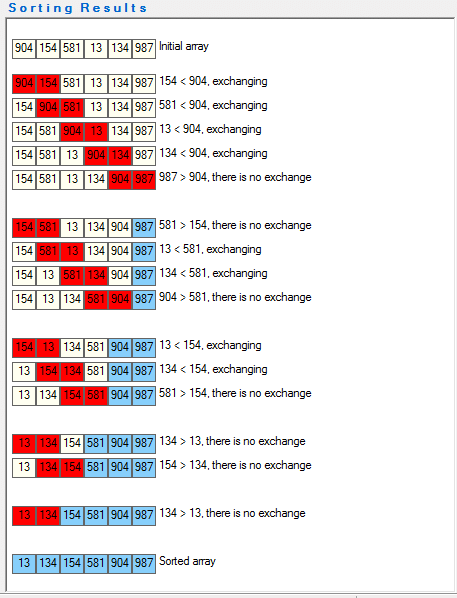
\includegraphics[scale=0.5]{img/Obtained-result-using-Bubble-sort-algorithm-and-array-with-six-elements.png}
    \caption{Corrida de Bubble Sort para un arreglo no ordenado (imagen sacada de Google).}
\end{figure}

A continuación, el código para el algoritmo de la burbuja\marginfootnote{Pseudocódigo sacado del Cormen.}:

\begin{algoritmo}
    \caption{Bubble Sort}\label{alg:bubble}
    \KwData{$A$ arreglo no ordenado}
    \KwResult{$A$ arreglo ordenado}
    \For{$i \leftarrow 1$ \textup{hasta} $length[A]$}{
        \For{$j \leftarrow length[A]$ \textup{hasta} $i+1$}{
        \If{$A[j] < A[j-1]$}{
        intercambia $A[j] \rightleftarrows A[j-1]$
        }
        }
    }
\end{algoritmo}

\break

Analicemos el algoritmo. Las operaciones son comparaciones e intercambio de valores. Así que, si el conjunto tiene $n$ elementos y esa es la medida de la instancia:

\begin{itemize}
    \item Para cada $j$ se hacen $n - j - 1$ comparaciones.
    \item Son $(n-1) + (n-2) + \dots + 2 + 1 = \frac{1}{2}n(n-1)$.
    \item Esto es $O(n^2)$.
    \item La cantidad de intercambios es también $O(n^2)$ (esto en el peor de los casos, se hace un intercambio después de cada comparación).
\end{itemize}

\textbf{En conclusión:} El algoritmo de la burbuja tiene eficiencia $O(n^2)$ en función de la cantidad de elementos del conjunto a ordenar.

Comparemos el algoritmo de la burbuja con una versión del algoritmo de inserción. El \textbf{algoritmo de inserción} construye una lista comenzando con el primer elemento del conjunto dado. Luego agrega el segundo elemento a la lista \textit{en el lugar correcto}. Y así sigue con los demás elementos del conjunto de manera que cada lista queda ordenada de una vez. La eficiencia de este algoritmo depende del método que se utilice para insertar el elemento \textit{en el lugar correcto}.

En nuestro caso, usaremos el método de \textbf{bisección}: Para insertar el $i$-ésimo elemento, se decide en cuál mitad de la lista debería ir. Después, en cuál mitad de esa mitad debería ir y así sucesivamente.

Ahora, analicemos este algoritmo:

\begin{itemize}
    \item Supongamos que el conjunto a ordenar tiene $n$ elementos.
    \item Si $n$ está entre $2^{r-1}$ y $2^r$, entonces hay que hacer $r$ comparaciones.
    \item En total son $\log_22 + \log_23 + \dots + \log_2 n$ comparaciones (aprox.).
    \item Esto es $O(n\log n)$.
\end{itemize}

\textbf{En conclusión}: El algoritmo de inserción, usando el método de bisección tiene eficiencia $O(n \log n)$. Pero al hacer la inserción en el lugar correcto, en el peor de los casos hay que intercambiar los términos de la lista. Esto serían otra vez $n^2$ intercambios. Por tanto, este algoritmo tiene también eficiencia $O(n^2)$.
Lo que hemos hecho es probar un caso particular de un resultado que se le debe a F.P Ramsey. Enunciemos el teorema de Ramsey de la siguiente manera:

\begin{teo}[Ramsey (TR)]\label{teo:TR}
    Para todo $n \in \N$ y todo $k \in \N$
    
    \[
    \omega \rightarrow (\omega)_r^n
    \]
\end{teo}

\begin{proof}
    Procedamos igual que en la demostración anterior con un argumento inductivo: El caso $r=1$ es trivial, así que pasemos a demostrar el caso $r=2$ con inducción sobre $n$.
        
    Si $n=1$, nuevamente es trivial; si $n=2$, ya hemos hecho la demostración en \ref{pre:ramsay1}. Supongamos entonces que el teorema vale para $n$ y probemos para $\omega \rightarrow (\omega)_2^{n+1}$. Como $\N$ es un conjunto infinito numerable, estudiar sus coloraciones vale para cualquier conjunto infinito numerable, así que por conveniencia nos quedaremos estudiando $\N$. Luego, tendremos $f: \N \rightarrow 2$, y nuestro objetivo será conseguir un conjunto homogéneo para $f$.
    
    \begin{marginfigure}
        \centering
        \begin{forest}
            [$0$, for tree={grow=90}, red
                [$1$, red
                    [\vdots
                        [$n-1$, red
                            [$X_1$
                                [$Y_3$
                                    [\vdots]
                                ]
                                [$Y_2$
                                    [\vdots]
                                ]
                            ]
                            [$X_0$
                                [$Y_1$
                                    [\vdots]
                                ]
                                [$Y_0$
                                    [\vdots]
                                ]
                            ]
                        ]
                    ]
                ]
            ]
        \end{forest}
        \caption{Representación de la construcción del árbol construído en la demostración del teorema de Ramsey.}
        \label{fig:ramseyfig1}
    \end{marginfigure}
    
    Entonces, construyamos un árbol de la siguiente manera: Sabemos que los primero $n$ elementos tienen el mismo color, es decir $f(n-1) = i$, donde $i = 0$ o $i = 1$. Definamos entonces dos particiones de $\N$, $X_0$ y $X_1$ tales que
    
    \[
    t \in X_i \iff f\left( n \cup \{t\} \right) = i, \quad i \in \{0,1\}
    \]
      
    \noindent ahora, partiremos ambos conjuntos $X_0$ y $X_1$ de la siguiente manera: Sea $t_0 \in X_0$ el menor elemento de $X_0$ y consideremos $C_{t_0} = \pred(t_0) \cup \{t_0\}$, definiremos dos conjuntos $Y_0$ y $Y_1$ tales que
    
    \[
    t \in Y_i \iff f\left( x \cup \{t\} \right) = i, \quad \forall x \in C_{t_0}^{[n]}
    \]
    
    Supongamos que en este árbol que hemos estado construyendo, tenemos en el nivel $m$ a un elemento $s$, ¿cómo es la partición del conjunto al que pertenece?. Pues consideremos $C_{s} = \pred(t_0) \cup \{s\}$ y sean entonces $Z_0$, $Z_1$ dichas particiones definidas de esta manera:
    
    \[
    t \in Z_i \iff f\left( x \cup \{t\} \right) = i, \quad \forall x \in C_{s}^{[n]}
    \]
    
    Los sucesores inmediatos de $s$ son elegidos de tal forma que tomamos el menor de cada $Z_i$. Entonces cada elemento del nivel $m$ tiene a lo sumo $2^{\binom{m}{n}}$ sucesores inmediatos, ya que para cada elemento del nivel $m$, $\left| C_s^{[n]} \right| = \binom{m}{n}$ y tenemos 2 colores.
    
    Para cada uno de los pares de particiones que hemos construído, puede ocurrir que uno de ellos sea vacío, pero no que los dos sea vacío. Esto es así por la cardinalidad de $\N$.
    
    Como resultado, hemos construído inductivamente un árbol $T$ infinito donde cada nivel es finito, entonces por el teorema \ref{teo:arboles1}, existe una rama $R \subset T$ infinita. Ahora, sea $x \in R^{[n]}$, para todo $s > n$, $t > s$, por construcción tenemos que
    
    \[
    f\left(x \cup \{s\}\right) = f\left(x \cup \{t\}\right)
    \]
    
    Con esto, podemos definir una nueva partición $g: R^{[n]} \rightarrow 2$, donde
    
    \begin{gather*}
        g(x) = 0, \quad \text{si} \quad f(x) = 0 \\
        g(x) = 1, \quad \text{si} \quad f(x) = 1
    \end{gather*}
    
    Luego, recordemos que por hipótesis inductiva, $\omega \rightarrow (\omega)_2^{n}$ y $g$ cumple las condiciones para la hipótesis inductiva. De esta manera, hay un $H \subset R$ infinito tal que $H^{[n]}$ es monocromático para $g$, y por lo tanto monocromático para $f$.
    
    De esta forma, hemos demostrado el caso $r=2$. Supongamos ahora que el teorema es válido para $r \leq k$, es decir que $\omega \rightarrow (\omega)_r^n$ es válido para todo $n$. Sea ahora $f: \N^{[n]} \rightarrow k+1$, podemos definir otra partición auxiliar $G: \N^{[n]} \rightarrow 2$ definida como
    
    \begin{gather*}
        G(x) = 0, \quad \text{si} \quad f(x) = 0 \\
        G(x) = 1, \quad \text{si} \quad f(x) = 1
    \end{gather*}
    
    \noindent entonces, por hipótesis inductiva, $G$ tiene un conjunto homogéneo $H$ infinito. Si $G\left( H^{[n]} \right) = 0$, $H$ es homogéneo para $f$. Si $G\left( H^{[n]} \right) = 1$, entonces $f|H^{[n]}$ es una partición de $k$ partes, y por hipótesis inductiva existe un conjunto $H' \subseteq H$ tal que es infinito y homogéneo. Este conjunto $H'$ también es homogéneo para $f$.
\end{proof}

Con esto demostrado, podemos pasar a demostrar una consecuencia de carácter finita del teorema de Ramsey:

\begin{teo}[Teorema de Ramsey finito (TFR)]\label{teo:TRF}
    Dados números enteros positivos $n, r$ y $m$, existe un entero positivo $N$ tal que
    
    \[
    N \rightarrow (m)_r^n
    \]
\end{teo}

\marginnote{La versión que se usará durante el transcurso del curso es la verión infinita del \TR}.

\begin{proof}
    Supongamos que el teorema no se cumple, es decir que para cada $N \in \N$, existe una coloración $f_N: N^{[n]} \rightarrow k$ tal que $\forall x \in N^{[m]}$, $x^{[n]}$ \textbf{no} es homogéneo para $f_N$.
    
    Con esto, definamos una función $f: \N^{[n+1]} \rightarrow k$ tal que para cualquier sucesión de números naturales $\{a_0, a_1, \dots, a_n\}$ tenemos
    
    \[
    f\left( \{a_0, a_1, \dots, a_n\} \right) = f_{a_n} \left( \{a_0, a_1, \dots, a_{n-1}\} \right)
    \]
    
    \noindent es decir, $f$ asigna a una sucesión creciente de $n+1$ elementos, la coloración será la que le asigne $f_{a_n}$ a los primeros $n$ elementos de esa lista.
    
    Luego, el \hyperref[teo:TR]{TR} nos dice que existe un $H \subset \N$ infinito tal que $H$ es homogéneo para $f$, con $H = \{h_0, h_1, \dots \}$. De esta forma, un conjunto $h$ de $m$ elementos tal que $h \subset H$ es también homogéneo para $f_{h_m}$. Al hacer la restricción $f_N|f_{h_m}$, tenemos que $h$ es homogéneo. Esto es una contradicción, ya que habíamos supuesto que no hay homogéneos de tamaño $m$ para $f_N$.
    
    Por lo tanto, el teorema de Ramsey finito es cierto.
\end{proof}
\begin{teo}[Teorema de la función implícita, generalización de la versión 3]
    Sea $F: \R^{n+m} \rightarrow \R^m$ diferenciable y de clase $C^2$, donde $F = (F_1, \dots, F_m)$ y a su vez $F_i(x_1, \dots, x_n, z_1, \dots, z_m)$. Consideremos $p_0 = (x_0, z_0) \in \R^{n+m}$. Consideremos también para cada $i = 1, \dots m$, $\Delta$ de la siguiente manera
    
    \[
    \Delta =
    \renewcommand\arraystretch{2}
    \begin{vmatrix}
        \frac{\partial F_1}{\partial z_1} & \dots & \frac{\partial F_1}{\partial z_m} \\
        \vdots & \ddots & \vdots \\
        \frac{\partial F_m}{\partial z_1} & \dots & \frac{\partial F_m}{\partial z_m}
    \end{vmatrix}
    \]
    
    \noindent donde cada derivada está evaluada en el punto $p_0$.
    
    Si tenemos que $F(p_0) = 0$ y $\Delta(p_0) \neq 0$, entonces en un entorno de $p_0$ tendremos que el sistema
    
    \[
    \begin{cases}
        F_1(x_1, \dots, x_n, z_1, \dots, z_m) = 0 \\
        \vdots \\
        F_m(x_1, \dots, x_n, z_1, \dots, z_m) = 0
    \end{cases}
    \]
    
    \noindent define de forma implícita a las funciones $z_i = f_i(x_1, \dots, x_n)$ con $i = 1, \dots, m$.
    
    Además, tendremos para $k = 1, \dots, n$ y $j = 1, \dots, m$
    
    \[
    \dfrac{\partial z_j}{\partial x_k} = -\dfrac{\dfrac{\partial(F_1, \dots, F_m)}{\partial(z_1, \dots, z_{j-1}, x_k, \dots, z_m)}}{\dfrac{\partial(F_1, \dots, F_m)}{\partial(z_1, \dots, z_m)}}
    \]
\end{teo}

A continuación no demostraremos este último teorema porque los cálculos se hacen muy extensos, pero si discutiremos algunas aplicaciones del T.F.I.:

\begin{ejem}
    Sean una función $F: \R^3 \rightarrow \R$ y $p_o = (x_0, y_0, z_0)$ tal que $F(p_0) = 0$. Sean también $\partial_xF$, $\partial_yF$ y $\partial_zF$ continuas en un entorno de $p_0$. Entonces $F(x,y,z) = 0$ define implícitamente $z = f(x,y)$. Más aún, se puede decir que
    
    \[
    \frac{\partial z}{\partial x}(p_0) = - \frac{\partial_xF(p_0)}{\partial_zF(p_0)}
    \qquad
    \frac{\partial z}{\partial y}(p_0) = - \frac{\partial_yF(p_0)}{\partial_zF(p_0)}
    \]
    
    \noindent si $\partial_zF(p_0) \neq 0$.
    
    Entonces, si calculamos la ecuación del plano tangente, esta nos queda como
    
    \begin{align*}
        z - z_0 &= \frac{\partial f}{\partial x}(x_0,y_0)(x-x_0) + \frac{\partial f}{\partial y}(x_0,y_0)(y-y_0) \\
            &= \partial_zF(p_0)(z-z_0) + \partial_yF(p_0)(y-y_0) + \partial_xF(p_0)(x-x_0) = 0
    \end{align*}
\end{ejem}

\begin{ejem}
    También es muy utilizado en el estudio de las ecuaciones diferenciales ordinarias exactas. Este tema lo abordaremos más adelante.
\end{ejem}

\subsection{Teorema de la función inversa}
\stepcounter{subsec}

Este teorema al igual que el teorema de la función implícita es central en el curso de análisis. Se irá desarrollando poco a poco porque la demostración es bien extensa.

Primero, veremos un lema que además de ser muy útil para la demostración de este teorema, también se utiliza en la materia de ecuaciones diferenciales.

\begin{lem}[Lema de contracción]
    Sean $M \subseteq \R^n$ cerrado y $F: M \rightarrow M$ una función y $K \in (0,1)$ tales que
    
    \[
    \normaeuc{F(x) - F(y)} \leq K\normaeuc{x - y} \quad \forall x,y \in M
    \]
    
    Entonces $F$ tiene un $x_0 \in M$ tal que $F(x_0) = x_0$. Luego nos queda que la sucesión $\sucinf{F^n(x_0)}{n}$ es de Cauchy y converge a $x_0$.
\end{lem}

\begin{proof}
    Primero tenemos que por hipótesis, para cada $x \in M$ fijo y arbitrario
    
    \[
    \normaeuc{F^2(x) - F(x)} = \normaeuc{F(F(x)) - F(x)} \leq K\normaeuc{F(x) - x}
    \]
    
    Ahora, por inducción podemos decir que
    
    \[
    \normaeuc{F^{n+1}(x) - F^n(x)} \leq K\normaeuc{F^n(x) - F^{n-1}(x)} \leq K^n\normaeuc{F(x) - x}
    \]
    
    En lo particular esto nos dice que $\sucinf{F^n(x_0)}{n}$ es una sucesión acotada, ya que
    
    \begin{align*}
        \normaeuc{F^n(x) - x} &\leq \normaeuc{F^n(x) - F^{n-1}(x)} + \normaeuc{F^{n-1}(x) - F^{n-2}(x)} + \dots \normaeuc{F(x) - x} \\
            &\leq \LaTeXunderbrace{(K^{n-1} + K^{n-2} + \dots + K)}_{\text{converge a $\frac{1}{1-K}$}}\normaeuc{F(x) - x}
    \end{align*}
    
    Nuevamente por inducción tenemos que para $m,k \in \N$
    
    \[
    \normaeuc{F^{m+k}(x) + F^m(x)} \leq K^m\normaeuc{F^k(x) + x}
    \]
    
    Ahora, como el término $F^k(x) - x$ está acotado, entonces existe $N_0 \in \N$ tal que $n,m \geq N_0$ con $n = m+k$, entonces
    
    \[
    \text{si $m,m \geq N_0$} \quad \implies \quad \normaeuc{F^{m+k}(x) + F^m(x)} < \varepsilon
    \]
    
    \noindent esto lo podemos hacer porque $\limtoinfty{m}{k^m} = 0$ ya que $K \in (0,1)$.
    
    Por lo tanto, $\sucinf{F^n(x_0)}{n}$ es de Cauchy.
    
    Ahora sea $x_0 \in M$ tal que $x_0 = \limtoinfty{n}{F^n(x)}$. Entonces dado $\varepsilon > 0$, existe $N_1$ tal que
    
    \[
    \text{si $n \geq N_1$} \quad \implies \quad \normaeuc{x_0 - F^n(x)} < \varepsilon
    \]
    
    Por lo tanto, si $n \geq N_1$
    
    \[
    \normaeuc{F(x_0) - F^{n+1}(x)} \leq K\normaeuc{x_0 - F^n(x)} < K\varepsilon
    \]
    
    De esta manera, $\limtoinfty{n}{F^n(x)} = F(x_0)$. En consecuencia $F(x_0) = x_0$.
    
    Lo único que queda es ver que $x_0$ es único: Supongamos que existe $x_1 \in M$ tal que $F(x_1) = x_1$. Consideremos ahora lo siguiente
    
    \begin{align*}
        \normaeuc{x_0 - x_1} &= \normaeuc{F(x_0) - F(x_1)} \leq K\normaeuc{x_0 - x_1} \\
        &\implies \normaeuc{x_0 - x_1} < K\normaeuc{x_0 - x_1}
    \end{align*}
    
    \noindent con $K \in (0,1)$. Esto es una contradicción ya que $\normaeuc{x_0 - x_1} > K\normaeuc{x_0 - x_1}$. Luego no existe dicho $x_1$ y concluimos que $x_0$ es único.
    
    Y así queda demostrado el lema de contracción, que próximamente utilizaremos para la demostración del lema de la función implícita.
\end{proof}
\subsection{Coloración de vértices de un grafo}

\begin{prob}
    Suponga que queremos organizar 6 eventos de una hora en una convención, estos eventos son $v_1, v_2, v_3, v_4, v_5, v_6$, y entre la audiencia hay gente que quiere ir al mismo tiempo a:
    
    \break
    \begin{itemize}
        \item $v_1$ y $v_2$.
        \item $v_1$ y $v_4$.
        \item $v_3$ y $v_5$.
        \item $v_2$ y $v_6$.
        \item $v_4$ y $v_5$.
        \item $v_5$ y $v_6$.
        \item $v_1$ y $v_6$.
    \end{itemize}
    
    ¿Cuántas horas harán falta para que los eventos puedan darse sin chocar entre la audiencia?
    \end{prob}
    
    \begin{proof}[Solución]
    La situación general se puede representar mediante el siguiente grafo:
    
    \begin{figure}
    \centering
    \begin{tikzpicture}
        \GraphInit[vstyle=Welsh]
        \Vertices[unit=2]{circle}{$v_3$, $v_2$, $v_1$, $v_6$, $v_5$, $v_4$}
        \Edges($v_1$,$v_2$,$v_6$,$v_1$,$v_4$,$v_5$,$v_6$,$v_5$,$v_3$)
    \end{tikzpicture}
    \caption{Cada vértice de este grafo representa un evento, y cada lado un potencial choque.}
    \label{fig:nocolor}
    \end{figure}
    
    \noindent donde los vértices representan los eventos y los lados representan los potenciales choques. El problema se resuelve al tomar los pares de vértices que \textbf{no} están conectados. Luego, una solución puede ser la siguiente:
    
    \begin{center}
        \begin{tabular}{cccc}
            \text{Hora 1} & \text{Hora 2} & \text{Hora 3} & \text{Hora 4} \\ \toprule
            $v_1$ \text{ y } $v_3$ & $v_2$ \text{ y } $v_4$ & $v_5$ & $v_6$
        \end{tabular}
    \end{center}
\end{proof}

En términos matemáticos, lo que hemos hecho es asignar una partición de cuatro partes al conjunto de vértices del grafo, con la condición de que ninguna de dichas partes contenga un par de vértices adyacentes.

A estas partes les llamamos \textbf{colores} en lugar de horas, pero la naturaleza exacta de los objetos no es importante.

\begin{defn}
    Sea $G=(V,L)$ un grafo. Una \ul{$r$-coloración} de $V$ es una función $f: V \rightarrow \{ 1, 2, \dots, r \}$ con $r \in \Nastk$ tal que $xy \in L \implies f(x) \neq f(y)$.
    
    La idea de este concepto será encontrar el mínimo $r$ tal que existe una $r$-coloración de los vértices de un grafo. Este es el \ul{número cromático}, y se representa con $\chi(G)$.
\end{defn}

De esta forma, si decidimos asignar un color a cada uno de los vértices del grafo \ref{fig:nocolor}, nos queda

\begin{figure}
    \centering
    \begin{tikzpicture}
        \GraphInit[vstyle=Welsh]
        \Vertices[unit=2]{circle}{$v_3$, $v_2$, $v_1$, $v_6$, $v_5$, $v_4$}
        \Edges($v_1$,$v_2$,$v_6$,$v_1$,$v_4$,$v_5$,$v_6$,$v_5$,$v_3$)
        \SetVertexNoLabel
        \AddVertexColor{red}{$v_1$,$v_3$}
        \AddVertexColor{blue}{$v_2$, $v_4$}
        \AddVertexColor{green}{$v_5$}
        \AddVertexColor{yellow}{$v_6$}
    \end{tikzpicture}
    \caption{El mismo grafo con la coloración planteada en la tabla.}
    \label{fig:color}
\end{figure}

\noindent sin embargo, este no es el menor número de colores que se pueden usar. Como los vértices $v_1$, $v_2$ y $v_6$ forman un triángulo, es decir, un grafo $K_3$, cada uno de ellos necesita un color distinto por ser adyacente a los otros dos, por lo que se necesitan al menos 3 colores para pintar el grafo completo.

\begin{figure}
    \centering
    \begin{tikzpicture}
        \GraphInit[vstyle=Welsh]
        \Vertices[unit=2]{circle}{$v_3$, $v_2$, $v_1$, $v_6$, $v_5$, $v_4$}
        \Edges($v_1$,$v_2$,$v_6$,$v_1$,$v_4$,$v_5$,$v_6$,$v_5$,$v_3$)
        \SetVertexNoLabel
        \AddVertexColor{red}{$v_1$}
        \AddVertexColor{blue}{$v_2$, $v_5$}
        \AddVertexColor{green}{$v_3$, $v_4$, $v_6$}
    \end{tikzpicture}
    \caption{Nuevamente el mismo grafo, pero utilizando menos colores.}
    \label{fig:color2}
\end{figure}

\begin{prob}
    ¿Cuál es el número cromático de un grafo cíclico $C_{2r}$ con un número par de vértices, y de uno $C_{2r+1}$ con un número impar de vértices?
\end{prob}

\begin{proof}[Solución]
    En el caso de los grafos cíclicos, si tenemos un ciclo par con una cantidad par de vértices, los vértices que tengan índice par tendrán un color distinto a los vecinos que tengan índice impar, pero como estos vértices se van turnando, con dos colores es suficiente para pintar el grafo. Si tenemos una cantidad impar de vértices, necesitaremos dos colores, y con ellos será suficiente para pintar $2r$ vértices, pero al agregar el vértice que falta, tendremos que este es vecino de un vértice con índice par, y de otro con vértice impar, por lo que necesitaremos un color adicional para pintar este último vértice, dándonos en total tres colores distintos.
\end{proof}

\begin{defn}
    Un grafo se dice que es \ul{bipartito} si se puede hallar una 2-partición de sus vértices tal que los vecinos de una están en la otra.
    
    Se tiene que, por definición
    
    \[
    \chi(G) = 2 \iff \text{$G$ es bipartito}
    \]
\end{defn}

Luego, si $G$ contiene un ciclo impar, entonces $\chi(G) \geq 3$. Por lo que podemos también decir que 

\[
\text{$G$ es bipartito} \implies \text{no hay ciclos impares en $G$}
\]

\begin{pre}
    ¿Si $G$ no tiene ciclos impares, entonces $\chi(G) = 2$?
\end{pre}
    
\begin{proof}[Respuesta]
    Sin pérdida de generalidad, supongamos que $G$ es conexo. Escojamos cualquier vértice y llamemoslo $v_1$ y diremos que está en el \textit{nivel 0}. Tomemos $v_2, \dots, v_r$, los vecinos de $v_1$ y diremos que están en el \textit{nivel 2}. Procediendo de esta forma, en el \textit{nivel $k$} habremos asignado todos los vértices adyacentes a los vértices del \textit{nivel $k-1$}, pero no aquellos del \textit{nivel $k-2$}.
    
    Al ordenar los vértices de esta forma, tendremos que los vértices en el \textit{nivel $k$} son adyacentes únicamente a los vértices del \textit{nivel $k-1$} y el \textit{nivel $k+1$}, y no a los del mismo nivel. Esto indica que, si tomamos dos vértices $x$ e $y$ en el mismo nivel, estos están unidos por un camino $m$ de igual longitud a cualquier vértice $z$ ubicado en algún nivel anterior, y los caminos se pueden elegir de forma tal que $z$ es el único vértice en común.
    
    Si $x$ e $y$ fuesen adyacentes, tendríamos que hay un ciclo de longitud impar $2m+1$, contrario a la hipótesis. Por lo tanto, si asignamos un color a los vértices de niveles pares, y otro a los vértices de niveles impares, tenemos $\chi(G)=2$.
    
    Y de esta forma, queda resuelto. La respuesta es afirmativa.
\end{proof}

Así, ya tenemos la demostración del teorema que enunciaremos a continuación.

\begin{teo}
    Un grafo es bipartito si y sólo si no contiene ciclos de longitud impar.
\end{teo}

\subsection{El algoritmo voraz}

Conseguir el número cromático de un grafo dado es un problema difícil. Sin embargo, si existe un método con el que construir una coloración de vértices utilizando una cantidad razonable de colores.

Este método consiste en asignar colores a los vértices en orden, de tal forma que cada vértice recibe el primer color que no haya sido asignado a uno de sus vecinos. En este algoritmo tomaremos la mejor desición que podamos en cada paso, sin tomar en cuenta si esta elección traerá problemas más adelante. Un algoritmo de este estilo se conoce como \textbf{algoritmo voraz}.

\begin{teo}
    Si $G$ es un grafo con máximo grado $k$, entonces
    
    \begin{enumerate}
        \item $\chi(G) \leq k+1$.
        \item Si $G$ es conexo y no regular, $\chi(G) \leq k$.
    \end{enumerate}
\end{teo}

\begin{proof}
    Pasemos a demostrar cada punto en orden:
    
    \begin{enumerate}
        \item Sean $v_1, \dots, v_n$ los vértices del grafo $G$. Entonces, para cualquiera de estos vértices, este tiene a lo sumo $k$ vecinos, por lo que el algoritmo voraz puede asignar a lo sumo $k$ colores a los vecinos de $v_i$. Por lo tanto, a $v_i$ se le asignará un color distinto. Y es en este sentido donde tenemos $k+1$ colores, por lo tanto $\chi(G) \leq k+1$.
        \item Como $G$ tiene grado máximo $k$ y no es regular entonces habrá al menos un vértice $v_n$ con grado menor a $k$. Entonces, tomemos en cuenta todos los vértices $v_{n-1}, v_{n-2}, \dots, v_{n-r}$ vecinos de $v_n$; hay a lo sumo $k-1$. Ahora, si consideramos los vecinos de $v_{n-1}$, tendremos a lo sumo $k-1$. Procediendo de manera sucesiva (y sin considerar los vértices que ya han sido considerados anteriormente), llegará un punto en el que consideraremos a todos los vértices del grafo $G$, ya que este está conectado. Como para cada uno de estos vértices se tienen a lo sumo $k-1$ vecinos, entonces procediendo con el algoritmo voraz tendremos a lo sumo $k-1$ colores para asignarle a cada uno. Si además contamos el color del vértice que estamos considerando, tendremos en total $k$ colores. Es en este sentido que tendremos $\chi(G) \leq k$.
    \end{enumerate}
    
    De esta forma, queda demostrado el teorema.
\end{proof}
\section{Teorema Fundamental del Cálculo y sus aplicaciones}

Ahora, desarrollaremos los resultados para establecer el Teorema Fundamental del Cálculo (TFC). Este teorema fue establecido por Leibniz y es el resultado que nos permite relacionar la teoría de derivadas con la teoría de integración. Este es el teorema central de la teoría de integración.

\begin{lem}
    Sea $f: [a,b] \rightarrow \R$ y $c \in (a,b)$. Si $f$ es integrable en $[a,c]$ y $[c,b]$ entonces $f$ es integrable en $[a,b]$.
\end{lem}

\begin{proof}
    Como la función es integrable en $[a,c]$, dado $\varepsilon > 0$, entonces existe una partición $P_1$ tal que
    
    \[
    U(f, P_1) - L(f, P_1) < \varepsilon/2
    \]
    
    \noindent análogamente, como $f$ es integrable en $[c,b]$, dado $\varepsilon > 0$, existe una partición $P_2$ tal que
    
    \[
    U(f, P_2) - L(f, P_2) < \varepsilon/2
    \]
    
    Ahora, definamos una partición $\Pe = P_1 \cup P_2$, sabemos que esta partición abarca al intervalo $[a,b]$ en su totalidad. Ahora, por \ref{eq:supamasb}, tenemos que
    
    \begin{gather*}
        U(f, \Pe) = U(f, P_1) + U(f, P_2) \\
        L(f, \Pe) = L(f, P_1) + L(f, P_2)
    \end{gather*}
    
    Así, tenemos que
    
    \[
    U(f, \Pe) - L(f, \Pe) = U(f, P_1) - L(f, P_1) + U(f, P_2) - L(f, P_2) < \varepsilon
    \]
    
    \noindent en consecuencia, la función $f$ será integrable en $[a,b]$.
\end{proof}

\begin{teo}
    Sea $f: [a,b] \rightarrow \R$ tal que $f \in \Rint$ y continua en $[a,b]$. Si $F(x) = \int_a^x f(t)dt$ para cada $x \in [a,b]$, entonces $F$\marginfootnote{Establecer esta función nos lleva a la siguiente definición:
    
    \begin{defn}
        Esta función $F$ definida de esta manera se conoce como la \ul{antiderivada} de $f$.
    \end{defn}} es continua en $[a,b]$.
\end{teo}

\begin{proof}
    Sea $\varepsilon > 0$, y los puntos $x_0, x$ en $[a,b]$ ($x > x_0$). Ahora, si queremos ver que $F$ es continua, para dicho $\varepsilon$ hemos de encontrar un $\delta$ tal que se satisfaga lo siguiente:
    
    \[
    \text{si} \quad |x - x_0| < \delta, \qquad \text{entonces} \quad |F(x) - F(x_0)| < \varepsilon
    \]
    
    Ahora, por el lema que acabamos de demostrar, y el teorema \ref{teo:riemod} tenemos
    
    \begin{align*}
        |F(x) - F(x_0)| &= \left| \int_a^x f(t)dt - \int_a^{x_0} f(t)dt \right| = \left| \int_a^x f(t)dt - \int_a^{x_0} f(t)dt \right| \\
        &= \left| \int_a^{x_0} f(t)dt + \int_{x_0}^x f(t)dt - \int_a^{x_0} f(t)dt \right| = \left| \int_{x_0}^x f(t)dt \right| \\
        &\leq \int_{x_0} |f(t)|dt
    \end{align*}
    
    \noindent como $f$ es continua y acotada en $[a,b]$, será acotada en $[x_0, x]$. Por lo tanto existe $M > 0$ tal que
    
    \[
    |F(x) - F(x_0)| \leq M\int_{x_0}^xdt \quad \text{con} \quad \sup_{x\in[a,b]} |f(x)|
    \]
    
    \noindent pero $M\int_{x_0}^xdt = M(x-x_0)$. Entonces, al escoger $\delta = \varepsilon/M$, tendremos que
    
    \[
    |F(x) - F(x_0)| \leq M(x-x_0) \leq M\delta = \epsilon
    \]
    
    De esta manera, queda demostrado.
\end{proof}

\begin{teo}[Primer Teorema Fundamental del Cálculo]\label{teo:1TFC}
    Sea una función $f: [a,b] \rightarrow \R$ con $f \in \Rint$ y continua. Entonces
    
    \[
    F(x) = \intab f(x)dx \quad \text{es derivable}
    \]
    
    Mas aún, $F'(x) = f(x)$.
\end{teo}

\begin{proof}
    En un principio, por definición,
    
    \[
    F'(x) = \lim_{x \to x_0} \frac{F(x) - F(x_0)}{x_0}
    \]
    
    \noindent es decir, que dado $\delta > 0$, queremos hallar un $\varepsilon > 0$ tal que
    
    \[
    \text{si} \quad |x - x_0| < \delta \quad \text{entonces} \left| \frac{F(x) - F(x_0)}{x-x_0} - f(x_0) \right| < \varepsilon
    \]
    
    \noindent entonces, estimemos cuánto da este último factor
    
    \[
    \left| \frac{F(x) - F(x_0)}{x-x_0} - f(x_0) \right| = \left| \frac{F(x) - F(x_0) - f(x_0)(x-x_0)}{x-x_0} \right|
    \]
    
    Por la definición de $F$, y el lema que acabamos de demostrar, tenemos
    
    \[
    \left|\dfrac{F(x) - F(x_0) - f(x_0)(x-x_0)}{x-x_0}\right| = \dfrac{\left| \int_{x_0}^x f(t)dt - \int_{x_0}^x f(x_0)dt  \right|}{|x-x_0|} \leq \dfrac{\int_{x_0}^x |f(t)dt - f(x_0)|}{|x-x_0|}
    \]
    
    Ahora, por la continuidad de $f$, dado $\epsilon > 0$, existe un $\delta_f > 0$ tal que si $|x-x_0| < \delta_f$ entonces $|f(x)-f(x_0)| < \epsilon$. Entonces
    
    \[
    \dfrac{\int_{x_0}^x |f(t)dt - f(x_0)|}{|x-x_0|} \leq \frac{\epsilon}{|x-x_0|}\int_{x_0}^xdt = \epsilon
    \]
    
    Por lo tanto, concluímos que si $|x-x_0| < \delta_f$, tenemos que
    
    \[
    \left| \frac{F(x) - F(x_0)}{x-x_0} - f(x_0) \right| < \varepsilon
    \]
    
    De esta manera, basta fijar $\delta = \delta_f$ para concluir que $F'(x_0) = f(x)$. Y así queda demostrado el teorema.
\end{proof}

\begin{teo}[Segundo Teorema Fundamental del Cálculo]\label{teo:2TFC}
    Sean $f \in C[a,b]$, $F$ tal que $F'(x) = f(x)$. Entonces
    
    \[
    \intab f(x)dx = F(b) - F(a)
    \]
\end{teo}

\begin{proof}
    Sea $G(x) = \int_a^x f(t)dt$, y por el 1TFC, obtenemos que $G'(x) = f(x)$. Pero por otro lado, también tenemos que $F'(x) = f(x)$. Como $G'(x) = F'(x)$ entonces
    
    \[
    G(x) - F(x) = k, \quad \text{con } k \in \R
    \]
    
    \noindent pero sabemos a qué equivale $G$, luego
    
    \[
    \int_a^x f(t)dt - F(x) = k \implies \cancelto{0}{\int_a^af(t)dt} - F(a) = k \implies -F(a) = k
    \]
    
    De esta manera,
    
    \begin{align*}
        \int_a^x f(t)&dt - F(x) = -F(a) \implies \intab f(t)dt - F(b) = -F(a) \\
        &\implies \intab f(t)dt = F(a) - F(b)
    \end{align*}
    
    \noindent y así queda demostrado el teorema.
\end{proof}

La primera aplicación importante que veremos de estos teoremas es una bastante usada en los cursos de cálculo:

\begin{teo}[Cambio de Variable]
    Sean $I_1, I_2 \subset \R$, y sean $f: I_1 \rightarrow I_2$ tal que $f \in C^1(I_1)$\marginfootnote{Aquí estamos manejando la siguiente notación:
    
    \begin{nota}
        Sea $f$ una función, e $I$ un intervalo cualquiera. Decir que $f \in C^1(I_1)$ equivale a pedir que la función sea continua, derivable y que su derivada sea continua sobre el intervalo $I$.
    \end{nota}}, $g: I_2 \rightarrow \R$ tal que $g \in C(I_2)$. Entonces
    
    \[
    \intab g\left(f(t)\right)f'(t)dt = \int_{f(a)}^{f(b)} g(u)du
    \]
\end{teo}

\begin{proof}
    Sea $G$ derivable en $I_2$ tal que $G'(x) = g(x)$. Luego, por 1TFC tenemos que $G(x) = \int_a^x g(u)du$, y por el 2TFC, podemos decir que
    
    \begin{equation}\label{eq:cl6.1}
        G(f(b))-G(f(a)) = \int_{f(a)}^{f(b)} g(u)du \quad \text{porque $G'(x) = g(x)$ para cada $x$}
    \end{equation}
    
    Por otro lado, la regla de la cadena nos dice que
    
    \[
    \left[ G(f(t)) \right]' = G'(f(t))f'(t)
    \]
    
    \noindent entonces, aplicando nuevamente el 2TFC,
    
    \begin{equation}\label{eq:cl6.2}
        \intab \left[ G(f(t)) \right]'dt = G(f(b)) - G(f(a))
    \end{equation}
    
    Luego, por \ref{eq:cl6.1} y \ref{eq:cl6.2} tenemos que
    
    \[
    \int_{f(a)}^{f(b)} g(u)du = \intab \left[ G(f(t)) \right]'dt = \intab g(f(t))f'(t)dt
    \]
    
    De esta forma, queda demostrado.
\end{proof}

\begin{teo}[Integración por partes]
    Sean $f, g \in C^1[a,b]$. Entonces
    
    \[
    \intab f(t)g'(t)dt = f(b)g(b) - f(a)g(a) - \intab f'(t)g(t)dt
    \]
\end{teo}

\begin{proof}
    Sabemos que
    
    \[
    [f(t)g(t)]' = f'(t)g(t) + g'(t)f(t)
    \]
    
    También sabemos por el 2TFC que
    
    \[
    \intab (f(t)g(t))'dt = f(b)g(b) - f(a)g(a)
    \]
    
    Por otro lado,
    
    \[
    \intab (f(t)g(t))'dt = \intab f'(t)g(t)dt + \intab g'(t)f(t)dt
    \]
    
    De esta forma, despejando y sustituyendo nos queda
    
    \begin{gather*}
        \intab g'(t)f(t)dt = \intab (f(t)g(t))'dt - \intab f'(t)g(t)dt \\
        \implies \intab g'(t)f(t)dt = f(b)g(b) - f(a)g(a) - \intab f'(t)g(t)dt
    \end{gather*}
    
    Así, queda demostrado el teorema.
\end{proof}
\subsection{Árboles y algoritmos de ordenamiento}

\begin{defn}
    Una aplicación muy frecuente del teorema \ref{teo:arbol1} es en el estudio de \ul{árboles de desición}, donde cada vértice interno representa una desición y los posibles resultados son representados por los lados. Los resultados finales los representan las hojas del árbol.
\end{defn}

Los algoritmos de ordenamiento revisados anteiormente resuelven el problema al comparar dos enteros y hacer la correspondiente transferencia de datos. Este procedimiento puede representarse como un árbol de desición donde cada vértice representa la comparación entre dos enteros $x$ e $y$, por lo que pueden haber dos resultados posibles, $x < y$ o $x > y$, dando como resultado un árbol binario.

Vimos anteriormente que Bubble Sort \ref{alg:bubble} e Insertion Sort son $O(n^2)$. Ahora veremos un algoritmo llamado \textbf{heapsort}. Este algoritmo es $O(n \log n)$ y hace uso de los árboles para mejorar su eficiencia. Para utilizar este algoritmo, tendremos que representar a los elementos a ordenar como un árbol binario y esto puede hacerse de la siguiente manera:

\begin{marginfigure}
    \centering
    \begin{forest}
    for tree={circle, draw}
    [$x_1$
        [$x_2$
            [$x_4$
                [$x_8$][$x_9$]]
            [$x_5$
                [$x_{10}$]
                [$x_{11}$]]]
        [$x_3$
            [$x_6$
                [$x_{12}$]]
            [$x_7$]]]
    \end{forest}
    \label{fig:pila1}
    \caption{Ejemplo para $n=12$.}
\end{marginfigure}

\vspace{15pt}

\begin{itemize}
    \item Se asignan los miembros de la lista $\{x_1, x_2, \dots, x_n\}$ a ordenar así: Asignamos $x_1$ a la raíz, $x_2$ será el primer hijo de $x_1$ y $x_3$ el segundo, $x_4$ será el primer hijo de $x_2$ y $x_5$ el segundo. Y así sucesivamente.
    \item Siguiendo de esta manera tendremos que el vértice $x_r$ es el padre de $x_{2r}$ y de $x_{2r+1}$. Cuando $n$ es par, el vértice $x_{n/2}$ tiene un único hijo: el vértice $x_n$. Así, hemos construído un árbol binario.
\end{itemize}

Ahora, heapsort tiene dos etapas: Primero, la lista sin ordenar se coloca en un \textit{pila}\marginfootnote{Pasemos a definir una pila:

\begin{defn}
    Una \ul{pila} es una estructura de datos cuya característica principal es que cada padre es menor que sus hijos, es decir que
    
    \[
    x_{2r} < x_{2r} \quad \wedge \quad x_{2r} < x_{2r+1}
    \]
\end{defn}}, y luego dicha pila se transforma en la lista ordenada.

Para la primera etapa, consideremos a los padres en orden inverso: Supongamos que al pararnos en $x_r$, ambos subárboles generados en $x_{2r}$ y $x_{2r+1}$ ya han sido convertidos en pilas. Si $x_r < x_{2r}$ y $x_r < x_{2r+1}$ no hay nada que hacer pues el subárbol que tenemos en $x_{2r}$ ya es una pila. De lo contrario, se intercambian los vértices y se vuelve a comparar e intercambiar para $x_r$ y $x_{4r}$, $x_{4r+1}$. Al llegar a una hoja, ya deberíamos encontrar un sitio donde $x_r$ quede fijo.

Esta regla para formar una pila forma la base para un procedimiento \textbf{pila}$(k,n)$, el cual dado un vértice $x_k$ con la propiedad de que los subárboles con ráiz en $x_{2k}$ y $x_{2k+1}$ son pilas, y hace que el subárbol que parte en $x_k$ sea una pila.

Ahora, en cualquier pila, la raíz siempre tendrá el menor valor, así que va en el primer luegar de la lista ordenada. Luego se sustituye dicho valor en la pila por el de $x_n$, por lo que tendremos un árbol fon $n-1$ vértices donde $x_2$ y $x_3$ son raíces de subárboles que son pilas, por lo que la llamada \textbf{pila}$(1,n-1)$ restaurará la propiedad de pila. Ahora la raíz tiene el menor valor y va en el segundo lugar de la lista ordenada. Y así sucesivamente.

\begin{algoritmo}
    \caption{heapsort}\label{alg:pila}
    \KwData{$\{x_1, \dots, x_n\} \quad$ arreglo no ordenado}
    \KwResult{$\{y_1, \dots, y_n\} \quad$ arreglo ordenado}
    \For{$j \leftarrow 0$ \textup{to} $\lfloor n/2 \rfloor - 1$}{
        \textbf{pila}$(\lfloor n/2 \rfloor - j, n)$
    }
    \For{$i \leftarrow 1$ \textup{to} $n-2$}{
        $y_i \leftarrow x_1; \quad x_1 \leftarrow x_{n-i+1}$ \\
        \textbf{pila}$(1, n-i)$
    }
    $y_{n-1} \leftarrow x_1; \quad y_n \leftarrow x_2$ 
\end{algoritmo}
\section{Clase 8}
\subsection{Resolución de Ecuaciones no homogéneas: Método de Variación de Parámetros}

Antes de pasar a explicar este método, hacen falta un par de teoremas\footnote{La demostración de estos dos teoremas puede encontrarse en el capítulo 3 del Boyce, y son necesarios para los resultados que se establecerán a continuación.} previos:

\begin{teo}
    Si $Y_1$, $Y_2$ son soluciones de la ecuación no homogénea \refeq{eq:edon1}, entonces la diferencia $Y_1 - Y_2$ es una solución a la ecuación homogénea asociada. Más aún, si $y_1$, $y_2$ conforman un conjunto fundamental de soluciones\footnote{Es decir, que $y_1(x)$ y $y_2(x)$ son soluciones a la ecuación y su Wronskiano es distinto de cero.} Entonces

    \[
        Y_1(x) - Y_2(x) = c_1y_1(x) + c_2y_2(x)
    \]

    \noindent con $c_1, c_2$ constantes.
\end{teo}

\begin{teo}
    La solución general de \ref{eq:edon1} puede escribirse en la forma

    \[
        y = \phi(x) = c_1y_1(x) + c_2y_2(x) + Y
    \]

    \noindent donde $y_1, y_2$ conforman un conjunto fundamental de soluciones de la ecuación homogénea asociada, $c_1, c_2$ son constantes, e $Y$ es una solución en específico de \ref{eq:edon1}.
\end{teo}

Recordemos que una ecuación diferencial no homogénea es aquella de la forma \refeq{eq:edon1}. La idea del método de Variación de Parámetros, es encontrar primero una solución a la ecuación homogénea asociada

\[
    y_c(x) = c_1y_1 + c_2y_2 = 0
\]

La idea básica es reemplazar las constantes $c_1$ y $c_2$ por funciones $u_1(x)$, $u_2(x)$ respectivamente, y hallar estas funciones de tal forma que la expresión

\[
    y = u_1y_1 + u_2y_2
\]

Es una solución de \ref{eq:edon1}.

\textbf{(!!!!) Toda esta charla que viene de $y'$ y $y''$ no la entendí muy bien, y tampoco entiendo muy bien qué es lo que se concluye. PREGUNTAR.}

Desarrollando esta idea, derivemos $y$ para hallar $u_1$ y $u_2$ en el proceso:

\begin{equation*}
    \begin{aligned}
        y' &= u_1'y_1 + u_2'y_2 + u_2y_2' + u_1y_1' \\
        y'' &= u_1''y_1 + u_1'y_1' + u_2''y_2 + u_2'y_2' + u_2'y_2' + u_2y_2'' + u_1'y_1' + u_1y_1''
    \end{aligned}
\end{equation*}

Como $y_1$, $y_2$ son soluciones de la ecuación homogénea asociada, Entonces

\[
    u_1'y_1 + u_2'y_2 = 0
\]

Y esto implica que

\begin{equation*}
    \begin{aligned}
        y' &= u_2y_2' + u_1y_1' \\
        y'' &=  u_1'y_1' + u_2'y_2' + u_2y_2'' + u_1y_1''
    \end{aligned}
\end{equation*}

Luego, gracias a los teoremas visto al inicio de la sección, sabemos que

\[
    f(x) = \LaTeXunderbrace{u_1(y_1'' + py_1' + qy_1) + u_2(y_2'' + py_2' + qy_2)}_{\text{Solución a la ecuación homogénea asociada}} + \LaTeXoverbrace{u_1'y_1' + u_2'y_2'}^{\mathclap{\text{Solución específica de la ecuación no homogénea}}}\footnotemark
\]\footnotetext{Como $y_1, y_2$ conforman un conjunto fundamental de soluciones, entonces también $y_1', y_2'$ también conforman uno.}

Como $W(y_1, y_2) \neq 0$, todo esto nos da como resultado el sistema

\begin{equation}
    \begin{cases*}
        u_1'y_1 + u_2'y_2 = 0 \\
        u_1'y_1' + u_2'y_2' = f(x)
    \end{cases*}
\end{equation}

De donde

\[
    u_1' = -\frac{y_2f(x)}{W(y_1, y_2)} \qquad u_2' = \frac{y_1f(x)}{W(y_1, y_2)}
\]

Todo esto nos quiere decir que para resolver EDO de este tipo, basta con seguir los siguientes pasos:

\begin{enumerate}
    \item Calcular $y_c$.
    \item Calcular $W(y_1, y_2)$.
    \item Aplicar $u_1', u_2'$ y calcular sus integrales.
\end{enumerate}
Para este teorema, la hipótesis de convergencia uniforme es clave. Veremos a continuación como en general, el teorema no se cumple para la convergencia puntual.

\begin{ejem}
    Consideremos la siguiente sucesión de funciones sobre $D = [0,1]$:
    
    \[
    f_{n-1}(x) = \begin{cases}
                 2n \quad x \in (1/n, 2/n) \\
                 0  \quad \text{si no}
             \end{cases}
    \]
    
    \noindent con $n \geq 2$.
    
    Al analizar las gráficas, estas son muy parecidas a las de \ref{ejem:cp}, y nos daremos cuenta de que la gráfica tenderá a cero. Entonces
    
    \[
    \limtoinfty{n}{f_n(x)} = f(x) \quad \text{donde $f(x) \equiv 0$ para cada $x \in [0,1]$}
    \]
    
    Pero
    
    \[
    \int_0^1 f_n(x)dx = \int_{\frac{1}{n}}^{\frac{2}{n}} 2ndx = 2
    \]
    
    Por lo tanto $\limtoinfty{n}{\int_0^1 f_n(x)dx} = 2$ y $\int_0^1 \limtoinfty{n}{f_n(x)}dx = 0$.
\end{ejem}

\begin{cor}
    Sea $\sucinf{f}{n}$ una sucesión de funciones integrables en $[a,b]$, y supongamos que $\sumtoinfty{n=1}{f_n}$ c.u. Entonces
    
    \[
    \intab \left(\sumtoinfty{n=1}{f_n(x)}\right)dx = \sumtoinfty{n=1}{\intab f_n(x)dx}
    \]
\end{cor}

\begin{proof}
    Como $\sucinf{f}{n}$ son integrables Riemann-integrables, entonces por las propiedades de la integral de Riemann, $\sucinf{S}{N}$ son integrables. Como $\sumtoinfty{n=1}{f_n}$ c.u entonces existe $f$ tal que
    
    \[
    \limtoinfty{N}{S_N} = f \quad \text{uniformemente}
    \]
    
    Entonces
    
    \[
    \limtoinfty{N}{\intab S_N(x)dx} = \intab f(x)dx
    \]
    
    Y en conclusión,
    
    \[
    \intab \left(\sumtoinfty{n=1}{f_n(x)}\right)dx = \sumtoinfty{n=1}{\intab f_n(x)dx}
    \]
    
    Así, queda demostrado.
\end{proof}

\begin{ejem}
    Consideremos la siguiente sucesión sobre $D = [0,1]$: $f_n(x) = x^n$ con $n \geq 0$. En el ejemplo \ref{ej:x^n} vimos que
    
    \[
    \sumtoinfty{n=0}{x^n} = \frac{1}{1-x} \quad \text{para cada $x \in [0,1]$}
    \]
    
    Consideremos un $r \in [0,1]$ tal que $x < r$. Entonces
    
    \[
    \left| \sumtoinfty{n=0}{x^n} \right| \leq \sumtoinfty{n=0}{|x^n|} < \sumtoinfty{n=0}{r^n} \qquad \footnotemark
    \]\footnotetext{Como ejercicio, se plantea lo siguiente:
    
    \begin{ejer}
        Demostrar que $\left| \sumtoinfty{n=0}{x^n} \right| \leq \sumtoinfty{n=0}{|x^n|}$.
    \end{ejer}}
    
    Ahora, tenemos una serie numérica $\sumtoinfty{n=0}{r^n}$ que converge a $\frac{1}{1-r}$, y por el teorema \ref{teo:wei}, nos queda que $\sumtoinfty{n=0}{x^n}$ converge. Luego, podemos intercambiar integrales por series gracias al corolario que recién establecimos. Así, sea $y \in (0, r)$,
    
    \[
    -\ln(1-y) = \int_0^y \frac{dx}{1-x} = \int_0^y \left( \sumtoinfty{n=0}{x^n}\right)dx = \sumtoinfty{n=0}{\int_0^y x^ndx} = \sumtoinfty{n=0}{\frac{y^{n+1}}{n+1}}
    \]
    
    De esta forma, hemos obtenido el desarrollo en series de $-\ln(1-y)$. De la misma manera podremos obtener el desarrollo en series de muchas funciones elementales.
\end{ejem}

\begin{teo}
    Sea $\sucinf{f}{n} \subset C'[a,b]$\marginfootnote{Recordemos que $C'$ quiere decir que:
    
    \begin{enumerate}
        \item $f_n: [a,b] \rightarrow \R$.
        \item $f_n$ son continuas.
        \item $f'_n$ son continuas.
    \end{enumerate}}. Supongamos que
    
    \begin{itemize}
        \item $f'_n \xrightarrow[n \to \infty]{\text{c.u}} g$.
        \item $f_n \xrightarrow[n \to \infty]{\text{c.p}} g$.
    \end{itemize}
    
    Entonces $f_n \xrightarrow[n \to \infty]{\text{c.u}} f$ y $f' = g$.
\end{teo}

\begin{proof}
    Demostremos ambos puntos en orden:
    
    \begin{itemize}
        \item Por el 2TFC, dados $m,n \in \N$, $x \in [a,b]$, entonces
    
        \[
        f_n(x) - f_m(x) = \int_a^x (f_n - f_m)'(t)dt + (f_n - f_m)(a)
        \]
        
        Luego
        
        \begin{equation}\label{eq:suc1}
            \norma{f_n - f_m} = \sup_{x \in D} \left| f_n(x) - f_m(x) \right| \leq (b-a)\norma{(f_n - f_m)'} + \left| (f_n - f_m)(a) \right| \quad \footnotemark
        \end{equation}\footnotetext{Se sustituye lo que está en la expresión anterior por lo que tenemos en la norma, y se desarrolla para llegar a ese resultado.}
        
        Por otro lado, como $f'_n$ c.u, entonces es fuertemente Cauchy, y además $\limtoinfty{n}{f_n(a)} = f(a)$ por la c.p de $f_n$. Entonces dado $\varepsilon > 0$, existe un $N_1 \in \N$ tal que
        
        \[
        \norma{(f_n - f_m)'} < \frac{\varepsilon}{2(b-a)}
        \]
        
        \noindent y además, existe un $N_2 \in \N$ tal que
        
        \[
        \left| (f_n - f_m)(a) \right| < \frac{\varepsilon}{2}
        \]
        
        \noindent si $n, m \in \N$ tales que $n, m \geq N_0 = \max(N_1, N_2)$.
        
        Ahora, por \ref{eq:suc1} tenemos que
        
        \[
        \norma{f_n - f_m} \leq (b-a)\norma{(f_n - f_m)'} + \left| (f_n - f_m)(a) \right| < \frac{\varepsilon(b-a)}{2(b-a)} + \frac{\varepsilon}{2} = \varepsilon
        \]
        
        De esta forma, dado $\varepsilon > 0$ entonces existe un $N_0$ tal que si $n, m \geq N_0$ entonces $\norma{f_n - f_m} < \varepsilon$. En conclusión, $\sucinf{f}{n}$ cumple la condición de Cauchy, por lo tanto $f_n \xrightarrow[]{\text{c.u}} f$.
        
        \item Por el 2TFC, tenemos que para cada $n \in \N$,
        
        \[
        f_n(x) = \int_a^x f'_n(t)dt - f_n(a)
        \]
        
        De esta manera,
        
        \begin{gather*}
            f(x) = \limtoinfty{n}{f_n(x)} = \limtoinfty{n}{\left[ \int_a^x f'_n(t)dt - f_n(a) \right]} = \limtoinfty{n}{\int_a^x f'_n(t)dt} - \limtoinfty{n}{f_n(a)} \\
            = \int_a^x [\limtoinfty{n}{f'_n(t)}]dt - f(a) = \int_a^x g(t)dt - f(a)
        \end{gather*}
        
        Nuevamente, por el 1TFC lo anterior implica que $f'(x) = g(x)$.
    \end{itemize}
    
    Así, quedan demostrados ambos puntos.
\end{proof}

\begin{cor}\label{cor:poderosisimo}
    Sea $\sucinf{f}{n} \subset C'[a,b]$ tales que:
    
    \begin{enumerate}
        \item $\sumtoinfty{n=1}{f_n}$ c.p.
        \item $\sumtoinfty{n=1}{f'_n}$ c.u.
    \end{enumerate}
    
    Entonces $\sumtoinfty{n=1}{f_n}$ c.u y además
    
    \[
    \left( \sumtoinfty{n=1}{f_n(t)} \right)' = \sumtoinfty{n=1}{f'_n(x)} \quad \footnotemark
    \]\footnotetext{Como ejercicio queda la demostración del corolario \ref{cor:poderosisimo}. La demostración se logra haciendo el mismo argumento que en el teorema anterior, pero definiendo $S_N = f_1 + \dots + f_N$.}
\end{cor}

\subsection{Teorema de Stone-Weierstrass}

\begin{teo}[Stone-Weierstrass]
    Sea $f \in C[a,b]$, entonces existe una sucesión $\sucinf{P}{n}$ de polinomios en $[a,b]$ tal que $\norma{P_n - f} \xrightarrow[n \to \infty]{} 0$.
\end{teo}

\begin{proof}
    Como primera consideración, en lugar de realizar la demostración en $[a,b]$, la realizaremos en $[0,1]$, podemos hacer esto debido a que si consideramos una función $p(x): [a,b] \rightarrow [0,1]$ tal que
    
    \[
    p(x) = \frac{x-a}{b-a}
    \]
    
    \noindent entonces podemos tomar una composición $p \circ f$, donde $f$ está definida en $[a,b]$.
    
    \begin{marginfigure}
        \centering
        \begin{tikzpicture}
            \begin{axis}[
                axis x line = bottom,
                axis y line = left,
                domain=0:1.1,
                width=5cm,
                height=5cm,
                clip=false,
                xtick=\empty,
                ytick=\empty,
                every axis x label/.style={at={(ticklabel cs: 0.95,0)},
                anchor=north},
                every axis y label/.style={at={(ticklabel cs: 0.95,0)},
                anchor=north east},
                xlabel=$x$,
                ylabel=$y$,
                ]
                \addplot [mark=none, blue, smooth] coordinates { (0,0.5) (0.1,0.4) (0.25, 0.2) (0.6,0.6) (0.8,0.3) (1,0.4) };
                \addplot [mark=*, red] coordinates { (0,0.5) (1,0.4) };
                \node[] at (-13,295) {\footnotesize $f(0)$};
                \node[] at (115,200) {\footnotesize $f(1)$};
            \end{axis}
        \end{tikzpicture}
        \label{fig:stnwei1}
        \caption{\footnotesize Aquí describimos la situación que tenemos en la demostración. Tenemos $f(x)$ como la línea azul, y $L(x)$ como la línea roja.}
    \end{marginfigure}
    
    La otra consideración es que $f(0) = f(1) = 0$. Esto lo podemos hacer porque al tomar la recta $L(x)$ que pasa por $f(0)$ y $f(1)$, entonces
    
    \[
    L(x) = (f(1) - f(0))x - f(0)
    \]
    
    \noindent definamos entonces $h(x) = f(x) - L(x)$. Luego, $h(1) = h(0) = 0$. Lo que hemos hecho es transladar la función $f$, obteniendo una nueva función $h(x)$. De esta manera podemos tomar $f(1) = f(0) = 0$.
    
    Sean para $n \in \N$
    
    \[
    K_n(t) = \begin{cases}
        \dfrac{(1-t^2)^n}{C_n}& \quad \text{si} \quad |t| \leq 1 \\
        0& \quad \text{si} \quad |t| > 1
    \end{cases}
    \]
    
    \noindent donde $\displaystyle C_n = \int_{-1}^1 (1-t^2)^ndt$. Como $(1-t^2)^n$ es una función acotada, la integral dará como resultado un valor finito y positivo (ya que $|t| \leq 1$).\marginfootnote{Estos valores se llaman los núcleos de Landau.}
    
    \begin{marginfigure}
        \centering
        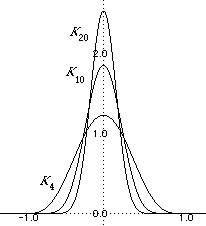
\includegraphics[scale=0.7]{img/landau.png}
        \label{fig:stnwei1}
        \caption{\footnotesize Aquí están representados los núcleos de Landau para algunos valores de $n$.}
    \end{marginfigure}
    
    Sea $z_n(t) = (1-t^2)^n$,
    
    \[
    z_n(-t) = (1-(-t)^2)^n = (1-t^2)^n = z_n(t)
    \]
    
    Por lo tanto, es una función par. Luego
    
    \[
    C_n = \int_{-1}^1 (1-t^2)^ndt = 2\int_0^1 (1-t^2)^ndt \geq 2\int_0^1 (1-t)^ndt = \frac{2}{n+1}
    \]
    
    Por otro lado, si definimos
    
    \[
    P_n(x) = \int_{\R} f(t)K_n(x-t)dt
    \]
    
    Lo primero que podemos notar es que $P_n$ son polinomios, porque $K_n(x-t)$ lo son. Esto es verificable gracias al binomio de Newton. Estimemos entonces cuánto vale $|P_n(x) - f(x)|$
    
    \[
    |P_n(x) - f(x)| = \left| \int_{\R} (f(x) - f(t))K_n(x-t)dt \right|
    \]
    
    \noindent ya que el valor de la integral de los $K_n$ es igual a $1$ \marginfootnote{Esto es porque
    
    \[
    \int_{-1}^1 K_n(t)dt = \frac{1}{C_n} \int_{-1}^1 (1-t^2)^ndt = 1
    \]}. Continuamos desarrollando
    
    \[
    \left| \int_{\R} (f(x) - f(t))K_n(x-t)dt \right| \leq \left| \int_{\R} (f(x) - f(t))\right| K_n(x-t)dt
    \]
    
    Hacemos ahora cambio de variable $u = x-t$. Entonces, lo anterior nos queda como
    
    \[
    \left| \int_{\R} (f(x-u) - f(x))\right| K_n(u)du
    \]
    
    Como $f$ es continua en $[0,1]$, el cual es compacto, entonces $f$ es uniformemente continua. Entonces dado $\varepsilon > 0$, existe un $\delta > 0$ tal que
    
    \begin{equation}\label{eq:stnwei1}
        \text{si} \quad |x-x-u| < \delta \implies |f(x) - f(x-u)| < \varepsilon
    \end{equation}
    
    Entonces, reescribiendo lo que teníamos antes, y separando la integral tenemos que
    
    \begin{gather}\label{eq:stnwei2}
        |P_n(x) - f(x)| \leq \notag \\
        \int_{|u| < \delta/2} \left|f(x-u) - f(x)\right|K_n(u)du + \int_{\delta/2 < |u| < 1} \left|f(x-u) - f(x)\right|K_n(u)du
    \end{gather}
    
    Por un lado, si $|u| < \delta/2$ y se cumple la hipótesis de continuidad, por \ref{eq:stnwei1} tendremos que
    
    \[
    \int_{|u| < \delta/2} \left|f(x-u) - f(x)\right|K_n(u)du \leq \varepsilon \int_{-1}^1 du = \varepsilon
    \]
    
    Y por el otro lado, como $K_n$ son funciones continuas y decrecientes en el intervalo $[\delta/2, 1]$, entonces para $\delta/2 < |u| < 1$, el máximo valor que pueden tomar es $K_n(\delta/2)$. Luego
    
    \begin{gather*}
        \int_{\delta/2 < |u| < 1} \left|f(x-u) - f(x)\right|K_n(u)du \leq K_n(\delta/2)\int_{\delta/2 < |u| < 1} \left|f(x-u) - f(x)\right|du \leq \\
        K_n(\delta/2)\int_{\delta/2 < |u| < 1} 2\norma{f}du = K_n(\delta/2)(2\norma{f})\int_{\delta/2 < |u| < 1}du \leq \\
        K_n(\delta/2)(2\norma{f})\int_{0 < |u| < 1}du = K_n(\delta/2)2\norma{f}
    \end{gather*}
    
    \noindent como los $K_n$ son integrables, conforman una sucesión que converge a cero al hacer $n \rightarrow \infty$. Entonces la expresión $\int_{\delta/2 < |u| < 1} \left|f(x-u) - f(x)\right|K_n(u)du$ puede hacerse tan pequeña como queramos.
    
    De esta forma, retomando lo que teníamos en \ref{eq:stnwei2}
    
    \begin{gather*}
        |P_n(x) - f(x)| < \varepsilon + 0 = \varepsilon \implies \\
        |P_n(x) - f(x)| \xrightarrow[n \to \infty]{} 0 \quad \forall x \in [0,1]
    \end{gather*}
    
    \noindent como el límite es igual a cero cuando $n$ tiene a infinito, pero no depende de $x$, podemos concluir que
    
    \[
    \norma{P_n - f} \xrightarrow[n \to \infty]{} 0
    \]
    
    De esta forma, queda demostrado el teorema.
\end{proof}
\subsection{Series de potencia. Región y radio de convergencia}

\begin{defn}
    Una \ul{serie de potencias} es una serie de funciones donde consideramos polinomios. Es decir que nos dedicaremos a estudiar expresiones de este tipo:

    \[
    \sumtoinfty{n=0}{a_n(x-a)^n}
    \]
    
    \noindent donde $\{a_n\}_{n=0}^{\infty} \subset \R$ es una sucesión de números reales. Al valor $a$ le llamamos \ul{centro}, y es el lugar alrededor del cual estamos desarrollando la serie de potencias.
\end{defn}

\begin{teo}
    Dada $\sumtoinfty{n=0}{a_nx^n}$ entonces solo una de las siguientes afirmaciones es cierta:
    
    \begin{itemize}
        \item $\sumtoinfty{n=0}{a_nx^n} < \infty$, $\forall x \in \R$.
        \item $\sumtoinfty{n=0}{a_nx^n} < \infty$ unicamente en $x=0$.
        \item Existe $R > 0$ tal que $\sumtoinfty{n=0}{a_nx^n} < \infty$ en $(-R, R)$.
    \end{itemize}
    
    Al valor $R$ se le conoce como el \ul{radio de convergencia}.
\end{teo}

Antes de demostrar este teorema, necesitaremos el siguiente lema:

\begin{lem}\label{lem:pot1}
    Si una serie de potencias $\sumtoinfty{n=0}{a_nx^n}$ converge en $x = x_0$ (con $x_0 \neq 0$) entonces la serie converge absolutamente\marginfootnote{Recordemos: Una serie $\sumtoinfty{n=0}{\beta_n}$ \ul{converge absolutamente} sii $\sumtoinfty{n=0}{|\beta_n|} < \infty$.} para cada $y$ tal que $|y| < |x_0|$.
\end{lem}

\begin{proof}
    Sabemos que la serie numérica $\sumtoinfty{n=0}{a_nx_0^n}$ converge, entonces
    
    \[
    \limtoinfty{n}{a_nx^n} = 0
    \]
    
    Luego existe $M > 0$ tal que
    
    \[
    |a_nx_0^n| < M \quad \forall n \in \N
    \]
    
    Ahora, si $|y| < |x_0|$ entonces
    
    \[
    |a_ny^n| = |a_nx_0^n|\left|\frac{y}{x_0}\right|^n \leq M\left|\frac{y}{x_0}\right|^n
    \]
    
    \noindent como esto se cumple para todo $n \in \N$, y además $\left|\frac{y}{x_0}\right| < 1$ por hipótesis, esto implica que
    
    \[
    \sumtoinfty{n=0}{|a_ny^n|} \leq M\sumtoinfty{n=0}{\left|\frac{y}{x_0}\right|^n} < \infty
    \]
    
    La serie converge para cada valor de $y$ porque tenemos una serie geométrica $\sumtoinfty{n=0}{r^n}$ con $0 < r < 1$\marginfootnote{Si $|y| > |x_0|$, la serie diverge.}, y es bien sabido que este tipo de series es convergente. Así, queda demostrado.
\end{proof}

\begin{proof}[Demostración del teorema]
    Si la serie converge en $x=0$, es trivial. Igualmente si la serie converge $\forall x \in \R$.
    
    Demostremos el tercer inciso. Queremos ver que $\sumtoinfty{n=0}{a_nx^n}$ converge para algún $R > 0$ si $|x| < R$ y diverge si $|x| > R$. Sean $x_0, x_1 \in \R$ (con $x_0 \neq 0$) tales que $\sumtoinfty{n=0}{a_nx_0^n} < \infty$ y $\sumtoinfty{n=0}{|a_nx_1^n|}$ diverge. Consideremos ahora un conjunto $S$ tal que
    
    \[
    S = \left\{ x \in \R : x > 0 \wedge \sumtoinfty{n=0}{a_nx^n} < \infty \right\}
    \]
    
    Vemos que $S \subseteq \R$ y además $S \neq \emptyset$ puesto que $x_0 \in S$. Y $S$ es acotado por lo siguiente: Supongamos que no es acotado. Entonces existe $x_2 \in \R$ tal que $x_2 > |x_1|$ con
    
    \[
    \sumtoinfty{n=0}{a_nx_2^n} < \infty
    \]
    
    Pero esto es contradicción por el lema \ref{lem:pot1} ya que estamos encontrando un valor más grande que $x_1$ para el cual la serie converge. Por lo tanto, $S$ es acotado.
    
    Por el axioma de completitud, $S$ tiene un supremo. Sea $R = \sup S$. Ahora, si $|x| < R$, existe $y \in S$ tal que
    
    \[
    |x| < y < R \quad \text{tal que} \quad \sumtoinfty{n=0}{a_ny^n} < \infty \implies \sumtoinfty{n=0}{|a_nx^n|} < \infty
    \]
    
    \noindent esto por el lema \ref{lem:pot1}.
    
    En conclusión, para todo $x \in (-R, R)$ la serie de potencias converge. Análogamente, si $|x| > R$ y al mismo tiempo que la serie converge, esto contradice el hecho de que $R$ es el supremo de $S$, por lo que tenemos una contradicción. Luego si $|x| > R$ la serie de potencias diverge.
    
    Así, queda demostrado el teorema.
\end{proof}

\begin{defn}
    El conjunto $S$ definido como en el teorema anterior se conoce como \ul{dominio de convergencia}.
\end{defn}

\subsection{Criterios de convergencia}

A continuación, veremos una serie de criterios para determinar la convergencia o divergencia de estas series. Estos criterios descansan fuertemente en los criterios vistos para series numéricas.

\begin{teo}[Criterio de Cauchy]\label{teo:critCauchy}
    Sean
    
    \[
    \sumtoinfty{n=0}{a_nx^n} \quad \text{y} \quad L = \limtoinfty{n}{\left|\frac{a_{n+1}}{a_n}\right|}
    \]
    
    Entonces
    
    \begin{enumerate}
        \item Si $L = \infty$ entonces la serie converge sólo en $x=0$.
        \item Si $L = 0$ entonces la serie converge $\forall x \in \R$.
        \item Si $0 < L < \infty$ entonces la serie converge absolutamente $\forall x$ tal que $|x| < R$ con $R = 1/L$.
    \end{enumerate}
\end{teo}

\begin{proof}
    Utilicemos el criterio del cociente para series numéricas, entonces
    
    \[
    \limtoinfty{n}{\left|\frac{a_{n+1}x^{n+1}}{a_nx^n}\right|} = |x| \limtoinfty{n}{\left|\frac{a_{n+1}}{a_n}\right|} = |x|L
    \]
    
    Si $|x|L < 1$ entonces la serie converge, y si $|x|L > 1$ entonces la serie diverge. Luego
    
    \[
    |x|L < 1 \iff |x| < 1/L \quad \text{y} \quad |x|L > 1 \iff |x| > 1/L
    \]
    
    \noindent en consecuencia la serie converge si $|x| < 1/L$ y diverge si $|x| > 1/L$. Cuando tenemos $|x| = 1/L$ el criterio no decide.
\end{proof}

\begin{ejem}
    Consideremos la serie
    
    \[
    \sumtoinfty{n=1}{(-1)^{n+1} \left(\frac{2}{3}\right) \frac{x^n}{n}}
    \]
    
    Entonces, el límite queda como
    
    \[
    \limtoinfty{n}{\left|\frac{a_{n+1}x^{n+1}}{a_nx^n}\right|} = \limtoinfty{n}{\left| \left(\frac{2}{3}\right)^{n+1}\left(\frac{n}{n+1}\right)\left(\frac{3}{2}\right)^n \right||x|} = \frac{2}{3}|x|\limtoinfty{n}{\cancelto{1}{\frac{n}{n+1}}} = \frac{2|x|}{3}
    \]
    
    Luego, $\frac{2}{3}|x| < 1$ sii $|x| < 3/2$. Por lo tanto, el radio de convergencia es $3/2$.
    
    ¿Qué pasa en los extremos?:
    
    \begin{itemize}
        \item Si $x = -3/2$, entonces la serie queda como
        
        \[
        \sumtoinfty{n=1}{(-1)^{2n+1} \left(\frac{2}{3}\right) \left(\frac{3}{2}\right)^n \frac{1}{n}} = -\sumtoinfty{n=1}{\frac{1}{n}}
        \]
        
        Y esta es la serie armónica, la cual diverge.
        
        \item Si $x = 3/2$, entonces la serie queda como
        
        \[
        \sumtoinfty{n=1}{(-1)^{n+1} \left(\frac{2}{3}\right) \left(\frac{3}{2}\right)^n \frac{1}{n}} = \sumtoinfty{n=1}{\frac{(-1)^{n+1}}{n}}
        \]
        
        Y esta es la serie alternada, la cual converge condicionalmente gracias al criterio de Leibniz\marginfootnote{Recordar de análisis 1 y cálculo 1.}.
    \end{itemize}
    
    De esta forma, la región de convergencia es $I = (-3/2, 3/2]$.
\end{ejem}

\begin{teo}[Criterio de la Raíz]\label{teo:raiz}
    Sea una serie de potencias $\sumtoinfty{n=0}{a_nx^n}$ y $L = \limtoinfty{n}{\sqrt[n]{|a_n|}}$. Entonces
    
    \begin{itemize}
        \item Si $L = \infty$ entonces la serie converge solo en $x=0$.
        \item Si $L=0$ entonces la serie converge $\forall x \in \R$.
        \item Si $0 < L < \infty$ la serie converge si $|x|<R$ con $R=1/L$.
    \end{itemize}
\end{teo}

\begin{proof}
    Primero, por propiedades de la potenciación, tenemos que
    
    \[
    \limtoinfty{n}{\sqrt[n]{|a_nx^n|}} = |x|\limtoinfty{n}{|a_n|} = |x|L
    \]
    
    Ahora, aplicando el criterio de la raíz para series númericas, la serie converge si $|x|L < 1$ y diverge si $|x|L>1$. Entonces, el radio de convergencia será de la forma $R=1/L$.
\end{proof}

\begin{ejem}
    Sea la serie
    
    \[
    \sumtoinfty{n=1}{\left(\frac{n+1}{n}\right)^{n^2}x^n}
    \]
    
    Entonces aplicando el criterio de la raíz,
    
    \[
    \limtoinfty{n}{\sqrt[n]{ \left| \left(\frac{n+1}{n}\right)^{n^2}x^n\right|}} = |x|\limtoinfty{n}{\left(1 + \frac{1}{n}\right)^n} = |x|e
    \]
    
    \noindent este último resultado porque tenemos un límite notable.
    
    Entonces, la serie converge para $|x| < 1/e$ y diverge en el complemento. Falta estudiar qué pasa en los extremos:
    
    \begin{itemize}
        \item Sea $x = 1/e$: Al sustituir, queda
        
        \[
        \sumtoinfty{n=1}{\left(\frac{n+1}{n}\right)^{n^2}\left(\frac{1}{e}\right)^n}
        \]
        
        Utilicemos el criterio de comparación. Sabemos que $e$ está acotado de la siguiente manera:
        
        \[
        \left(\frac{n+1}{n}\right)^n < e < \left(\frac{n+1}{n}\right)^{n+1} \quad \footnotemark
        \]\footnotetext{Esto se ve en el curso de análisis 1.}
        
        \noindent y esto para cada $n\geq1$. Luego, esto implica que
        
        \[
        \left(\frac{n}{n+1}\right)^n > 1/e > \left(\frac{n}{n+1}\right)^{n+1} \implies \left(\frac{n}{n+1}\right)^{n^2} > 1/e^n > \left(\frac{n}{n+1}\right)^{n^2+n}
        \]
        
        Multipliquemos lo anterior por el factor $\left(\frac{n+1}{n}\right)^{n^2}$ y nos queda
        
        \[
        1 > \left(\frac{n+1}{n}\right)^{n^2} 1/e^n > \left(\frac{n}{n+1}\right)^n \implies \sumtoinfty{n=1}{\left(\frac{n+1}{n}\right)^{n^2} 1/e^n} > \sumtoinfty{n=1}{\left(\frac{n}{n+1}\right)^n}
        \]
        
        Por otro lado
        
        \[
        \limtoinfty{n}{\left(\frac{n}{n+1}\right)^n} = \limtoinfty{n}{e^{\displaystyle n\ln\left(\frac{n}{n+1}\right)}} = e^{\displaystyle \limtoinfty{n}{n\ln\left(\frac{n}{n+1}\right)}} = 1/e
        \]
        
        \noindent este resultado es fácilmente verificable por L'Hopital.
        
        Como $\limtoinfty{n}{\left(\frac{n}{n+1}\right)^n} \neq 0$, el término general de la serie numérica no tiende a cero y por lo tanto la serie diverge.
        
        En conclusión la serie $\sumtoinfty{n=1}{\left(\frac{n+1}{n}\right)^{n^2}\left(\frac{1}{e}\right)^n}$ diverge.
        
        \item Sea $x = -1/e$. Estamos mirando ahora la siguiente serie
        
        \[
        \sumtoinfty{n=1}{(-1)^n\left(\frac{n+1}{n}\right)^{n^2}\left(\frac{1}{e}\right)^n}
        \]
        
        La cual es una serie alternada, pero como el factor $\left(\frac{n+1}{n}\right)^{n^2}\left(\frac{1}{e}\right)^n$ no tiende a cero por el mismo análisis que realizamos anteriormente. Luego los términos oscilan y nuevamente la serie diverge.
    \end{itemize}
    
    En conclusión, el radio de convergencia es $R=1/e$ y la región de convergencia es $(-1/e, 1/e)$.
\end{ejem}
\subsection{Convergencia uniforme para series de potencias}

\begin{teo}
    Sea $\sumtoinfty{n=0}{a_nx^n}$ con radio de convergencia $R > 0$. Sea $K \subset (-R,R)$ compacto. Entonces la serie c.u en $K$.
\end{teo}

\begin{proof}
    Primero, sea $x_0 \in K$ fijo, y como $K \subset (-R, R)$ entonces $|x_0|<R$. Sea $y \in K$ tal que $|y|<|x_0|$, en ese caso la serie $\sumtoinfty{n=0}{a_ny^n}$ converge absolutamente por \ref{lem:pot1}.
    
    Ahora, para cada $n \geq 0$ tenemos que
    
    \[
    |a_n||y|^n < |a_n||x_0|^n \coloneqq \beta_n \in \R \quad \text{con $\beta_n$ fijos}
    \]
    
    Esto implica que
    
    \[
    \sumtoinfty{n=0}{|a_n||y|^n} \leq \LaTeXunderbrace{\sumtoinfty{n=0}{\beta_n}}_{\text{convergente}}
    \]
    
    Luego por \ref{teo:wei} la serie $\sumtoinfty{n=0}{a_ny^n}$ c.u para todo $y \in K$ tal que $|y| < |x_0|$. Recordemos que $x_0$ es fijo, pero el mismo argumento lo podemos repetir para todo $x \in K$, entonces $\sumtoinfty{n=0}{a_ny^n}$ c.u para todo $y \in K$.
\end{proof}

\begin{teo}
    Sea $\sumtoinfty{n=0}{a_nx^n}$ con radio de convergencia $R>0$. Sea $f(x) = \sumtoinfty{n=0}{a_nx^n}$ para cada $x$ tal que $|x|<R$. Entonces $f$ es continua.
\end{teo}

\begin{proof}
    Sean $\varepsilon>0$ y $x,y \in (-R,R)$. Luego
    
    \[
    f(x) = \sumtoinfty{n=0}{a_nx^n} \quad \text{y} \quad f(y) = \sumtoinfty{n=0}{a_ny^n}
    \]
    
    Y también tenemos que
    
    \[
    \limtoinfty{N}{|S_N(x) - f(x)|} = 0 \quad \text{y} \quad \limtoinfty{N}{|S_N(y) - f(y)|} = 0 \quad \text{puntualmente}
    \]
    
    Luego existen $N_1, N_2 \in \N$ tales que si $n \geq \max(N_1, N_2)$
    
    \[
    |S_N(y) - f(y)| < \varepsilon/3 \quad \text{y} \quad |S_N(x) - f(x)| < \varepsilon/3
    \]
    
    Por otro lado, si $N \geq \max(N_1,N_2)$
    
    \[
    |S_N(x) - S_N(y)| \leq \sum_{k=0}^N |a_k||x^k-y^k|
    \]
    
    Y como
    
    \[
    |x^k-y^k| = |x-y||x^{k-1}+ x^{k-2}y + \dots + xy^{k-2} + y^{k-1}| \leq |x-y|\left|\sum_{j=0}^{k-1} x^j y^{k-j}\right| \leq |x-y|\sum_{j=0}^{k-1}|x|^j|y|^{k-j}
    \]
    
    De esta forma,
    
    \[
    |S_N(x) - S_N(y)| \leq |x-y| \sum_{k=0}^n |a_k| \left(\sum_{j=0}^{k-1}|x|^j|y|^{k-j}\right)
    \]
    
    Como $|x|<R$, $|y|<R$ nos queda que
    
    \[
    |x-y| \sum_{k=0}^n |a_k| \left(\sum_{j=0}^{k-1}|x|^j|y|^{k-j}\right) \leq |x-y|\left(\sum_{k=0}^N kR^k|a_k|\right)
    \]
    
    De esta forma, $\displaystyle |S_N(x) - S_N(y)| \leq |x-y|\left(\sum_{k=0}^N kR^k|a_k|\right)$
    
    Fijemos entonces $\displaystyle \delta = \dfrac{\varepsilon}{\displaystyle 3\left(\sum_{k=1}^N kR^k|a_k|\right)}$. Luego si $|x-y| < \delta$
    
    \begin{align*}
        |f(x) - f(y)| &= |f(x) - f(y) + S_N(x) - S_N(x) + S_N(y) - S_N(y)| \\
        &\leq |f(x) - S_N(x)| + |f(y) - S_N(y)| + |S_N(x) - S_N(y)| \\
        &< \frac{\varepsilon}{3} + \frac{\varepsilon}{3} + \dfrac{\displaystyle\varepsilon\left(\sum_{k=1}^N kR^k|a_k|\right)}{\displaystyle 3\left(\sum_{k=1}^N kR^k|a_k|\right)} = \varepsilon
    \end{align*}
    
    \noindent con $n \geq \max(N_1,N_2)$.
    
    Así, queda demostrada la continuidad de la función $f(x)$.
\end{proof}

\begin{teo}
    Sea $\sumtoinfty{n=0}{a_nx^n}$ con radio de convergencia $R$. Entonces $\sumtoinfty{n=1}{na_nx^{n-1}}$ tiene radio de convergencia $R$.
\end{teo}

\begin{proof}
    Antes de empezar la demostración como tal, necesitamos hacer una observación previa: Sean entonces
    
    \begin{gather*}
        \sumtoinfty{n=0}{a_nx^n} \quad \text{con radio $R_1$} \\
        \sumtoinfty{n=0}{na_nx^{n-1}} \quad \text{con radio $R_2$}
    \end{gather*}
    
    La desigualdad $|a_n| \leq n|a_n|$ para todo $n \in \N$ implica que $R_2 \leq R_1$: No puede ocurrir que $\sumtoinfty{n=0}{na_nx^{n-1}}$ converja y $R_2 > R_1$, ya que entonces podríamos tomar $x_1$ tal que $R_1 < |x_1| < R_2$ en cuyo caso puede ocurrir
    
    \begin{itemize}
        \item $\sumtoinfty{n=0}{a_nx_1^n}$ diverge pues $|x_1|>R_1$.
        \item $\sumtoinfty{n=0}{a_nx_1^n}$ converge por el criterio de comparación, pues $|a_n| \leq n|a_n|$ y $|x_1|<R_2$.
    \end{itemize}
    
    Pero esto es un absurdo ya que la serie converge y diverge al mismo tiempo, cosa que no puede pasar. En consecuencia, $R_2 \leq R_1$.
    
    Ahora, ¿por qué podemos decir que los radios son iguales? Evaluemos ambas series por el criterio de la razón:
    
    \[
    \limtoinfty{n}{\left|\frac{(n+1)a_{n+1}x^n}{na_nx^{n-1}}\right|} = |x|\limtoinfty{n}{\left(\frac{n+1}{n}\right)\left|\frac{a_{n+1}}{a_n}\right|}
    \]
    
    Como el radio de convergencia de la serie es $R$, entonces como vimos en \ref{teo:critCauchy} nos queda que
    
    \[
    \limtoinfty{n}{\left|\frac{a_{n+1}}{a_n}\right|} = L = 1/R
    \]
    
    En consecuencia
    
    \[
    \limtoinfty{n}{\left|\frac{(n+1)a_{n+1}x^n}{na_nx^{n-1}}\right|} = |x|L < 1 \iff |x| < \frac{1}{L} = R_1
    \]
    
    En conclusión, la serie $\sumtoinfty{n=1}{na_nx^{n-1}}$ tiene radio de convergencia $R$.
\end{proof}

De este resultado se desprende el siguiente corolario bastante importante.

\begin{cor}
    Si $f(x) = \sumtoinfty{n=0}{a_nx^n}$ para $x \in [-a,a] \subset (-R,R)$ con $R$ el radio de convergencia de la serie. Entonces
    
    \[
    f'(x) = \sumtoinfty{n=1}{na_nx^{n-1}}
    \]
    
    para todo $x \in [-a,a] \subset (-R,R)$.
    
    Es decir, podemos intercambiar series con derivadas.
\end{cor}

Y esto nos va a permitir resolver problemas muy propios de cursos de cálculo como el siguiente:

\begin{ejem}
    Demostrar que
    
    \[
    \sumtoinfty{n=1}{nx^n} = \frac{x}{(1-x)^2} \quad \text{si $|x|<a<1$}
    \]
\end{ejem}

\begin{proof}[Solución]
    Partimos de lo siguiente
    
    \[
    \sumtoinfty{n=1}{nx^n} = x\left[ \sumtoinfty{n=0}{xn^{n-1}} \right] = x\left[\sumtoinfty{n=0}{x^n}\right]'
    \]
    
    Como hemos visto anteriormente, $\sumtoinfty{n=0}{x^n} = \frac{1}{1-x}$ ya que $|x|<a<1$. Entonces
    
    \[
    x\left[\sumtoinfty{n=0}{x^n}\right]' = x\left[\frac{1}{1-x}\right]' = \frac{x}{(1-x)^2}
    \]
    
    De esta forma, queda demostrado.
\end{proof}

\subsection{Álgebra de series de potencias}

\begin{teo}\label{teo:alge1}
    Sean las series $f(x) = \sumtoinfty{n=0}{a_nx^n}$, $g(x) = \sumtoinfty{n=0}{b_nx^n}$ con radio de convergencia común $R > 0$. Entonces
    
    \[
    \sumtoinfty{n=0}{a_nx^n} + \sumtoinfty{n=0}{b_nx^n} = \sumtoinfty{n=0}{(a_n+b_n)x^n} = f(x) + g(x)
    \]
\end{teo}

\marginnote{La demostración del teorema \ref{teo:alge1} queda como ejercicio.}

\begin{teo}
    Sean las series $f(x) = \sumtoinfty{n=0}{a_nx^n}$, $g(x) = \sumtoinfty{n=0}{b_nx^n}$ con radios de convergencia $R_1$, $R_2 > 0$ respectivamente. Entonces
    
    \[
    \left(\sumtoinfty{n=0}{a_nx^n}\right)\left(\sumtoinfty{n=0}{b_nx^n}\right) = \left(\sumtoinfty{n=0}{c_nx^n}\right)
    \]
    
    \noindent donde $c_n = \sum_{k=0}^n a_kb_n-k$, con $n = 0,1,\dots$, y radio de convergencia $R < min(R_1,R_2)$.
\end{teo}

\begin{proof}
    Consideremos $N \in \N$. Luego sean
    
    \[
    S_N^a(x) = \sum_{n=0}^N a_nx^n, \quad S_N^b(x) = \sum_{n=0}^N b_nx^n, \quad S_N^c(x) = \sum_{n=0}^N c_nx^n
    \]
    
    Definamos también
    
    \[
    d_N(x) = g(x) - S_N^b(x) \quad \text{para cada $x$ tal que $|x|<R$}
    \]
    
    \noindent y 
    
    \[
    e_N = \sum_{n=0}^{N}a_nx^nd_{N-n}
    \]
    
    Ahora, para cada $M \in \N$ se tiene que
    
    \[
    S_M^c(x) = \sum_{n=0}^M \left(\sum_{k=0}^na_kb_{n-k}\right)x^n = \sum_{n=0}^M \left(\sum_{k=0}^n \LaTeXunderbrace{a_kb_{n-k}x^{n-k}}_{=f_n(k)} \right) = \sum_{n=0}^M \left(\sum_{k=0}^M f_n(k)\right)
    \]
    
    \noindent donde
    
    \[
    f_n(x) = \begin{cases}
                 a_kx^kb_{n-k}x^{n-k} \quad n \geq k \\
                 0, \quad n < k
             \end{cases}
    \]
    
    Luego tenemos que las sumas parciales quedan como
    
    \[
    S_M^c(x) = \sum_{k=0}^M \sum_{n=0}^M f_n(x) = \sum_{k=0}^n \sum_{n=k}^M a_kx^kb_{n-k}x^{n-k} = \left( \sum_{k=0}^M a_kx^k \right)\left(\sum_{j=0}^{M-k} b_jx^j\right)
    \]
    
    De esta manera, nos queda que
    
    \[
    S_M^c = \sum_{k=0}^M a_kx^kS_{M-k}^b = \left(\sum_{k=0}^M a_kx^k (g-d_{M-k})\right) = gS_M^a - e_M
    \]
    
    Falta ver que $\limtoinfty{M}{e_M} = 0$. Entonces primero consideremos lo siguiente
    
    \[
    \limtoinfty{M}{d_M} = \limtoinfty{M}{g-S_M^b} = g - g = 0 \quad \text{para todo $x$ tal que $|x|<R$}
    \]
    
    Entonces dado $\varepsilon > 0$, existe $N_1 \in \N$ tal que si $n \geq N_1$,
    
    \[
    |d_n| < \frac{\varepsilon}{2k} \quad \text{con $k = \sumtoinfty{n}{|a_n||x^n|}$}
    \]
    
    \noindent como estamos trabajando para $|x|<R$ entonces las series $f(x)$, $g(x)$ convergen absolutamente, por lo que $k$ es una cantidad finita.
    
    Por otro lado, bajo la misma hipótesis de que las series convergen absolutamente, existe un $N_2 \in \N$ tal que si $n \geq N_2$,
    
    \[
    \sumtoinfty{n=N_2+1}{|a_nx^n|} < \frac{\varepsilon}{2\alpha}
    \]
    
    \noindent donde $\alpha > 0$ es tal que $|d_M| \leq \alpha$ para todo $M$. Esto se puede asegurar porque la sucesión $|d_M|$ converge a cero, entonces es acotada.
    
    Sea ahora $N_0 = \max(N_1, N_2)$. Si $M > 2N_0$ entonces
    
    \[
    |e_M| \leq \sum_{k=0}^N |b_k x^k \cancelto{\frac{\varepsilon}{2k}}{d_{M-k}}| + \sum_{k=N+1}^M |a_k x^k d_{M-k}| \leq \frac{\varepsilon}{2k}\left(\sumtoinfty{k=0}{|a_k x^k|}\right) + \alpha \left(\sumtoinfty{k=N+1}{|a_kx^k|}\right) \leq \varepsilon/2 + \varepsilon/2 = \varepsilon
    \]
    
    De esta forma, $\limtoinfty{M}{e_M} = 0$. Por lo tanto
    
    \[
    \limtoinfty{M}{S_M^c} = \limtoinfty{M}{gS_M^a - e_M} = fg \quad \text{si $|x|<R$}
    \]
    
    De esta forma, queda demostrado.
\end{proof}
\subsection{Teorema min-max}

A continuación describiremos un método para aumentar el valor de un flujo dado suponiendo que el flujo no tiene el máximo valor posible. Este método nos llevará a probar el teorema min-max (mínimo corte, máximo flujo).

Tomemos como ejemplo nuevamente la red \ref{fig:red} con el flujo descrito más adelante. En el camino dirigido $s, a, t$ vemos que ni el arco $(s,a)$ ni $(a,t)$ tienen flujos que tomen valores máximos para sus capacidades, por lo que podemos incrementar el flujo para ambos arcos hasta que la capacidad de uno de ellos sea alcanzada. Definimos entonces $f_1(s,a) = 4$ y $f_1(a,t) = 3$ y ahora $(a,t)$ está saturado. Definimos ahora $f_1(x,y)$ para el resto de los arcos y obtendremos un nuevo flujo

\begin{tabular}{c|ccccccccc}
    $(x,y)$  & $(s,a)$ & $(s,b)$ & $(s,c)$ & $(a,d)$ & $(b,d)$ & $(c,d)$ & $(a,t)$ & $(c,t)$ & $(d,t)$ \\
    $f(x,y)$ & $4$ & $2$ & $3$ & $1$ & $2$ & $1$ & $3$ & $2$ & $4$
\end{tabular}

\noindent con valor $\val(f_1) = \val(f) + 1 = f$.

Pero esto se puede mejorar: Sea $G$ el grafo base del grafo dirigido $D$ de la red y consideremos el camino $s, a, d, c, t$  en $G$. Para la red, el arco $(c,d)$ va en sentido contrario, entonces tendríamos el siguiente camino junto a sus flujos y capacidades en la red:

\[
s \xlongrightarrow[5]{4} a \xlongrightarrow[6]{1} d \xlongleftarrow[7]{1} c \xlongrightarrow[5]{2} t
\]

Como el flujo en $(c,d)$ está en dirección contraria al resto, podemos reducir su flujo en 1 e incrementar el flujo en el resto de los arcos por la misma cantidad sin violar la regla de conservación. En este sentido, obtenemos un nuevo flujo $f_2$ tal que sus valores en el camino descrito son

\[
s \xlongrightarrow[5]{5} a \xlongrightarrow[6]{2} d \xlongleftarrow[7]{0} c \xlongrightarrow[5]{3} t
\]

\noindent y el resto de los arcos tienen el mismo flujo que en $f_1$.

En este flujo ya no podemos seguir incrementando debido a que $(s,a)$ está saturado y el flujo en $(c,d)$ no puede ser menor que cero. Ahora $\val(f_2) = \val(f_1) + 1 = 10$. Sea el corte $S = \{s,b\}$, $T=\{a,c,d,t\}$, este corte tiene capacidad $c(S,T)=10$. Entonces por el teorema \ref{teo:cotavalor}, $f_2$ es un flujo máximo (en el sentido que tiene el máximo valor posbile).

En general, dado un flujo $f$ en una red con digrafo $D$ y grafo base $G$, decimos que un camino en $G$

\[
s=x_1,x_2,\dots,x_{k-1},x_k=t
\]

\noindent es un \ul{camino que aumenta} $f$ si para $i \leq k-1$ se cumple que

\begin{gather*}
    (x_i, x_{i+1}) \in A(D) \implies f(x_i,x_{i+1}) < c(x_i,x_{i+1}) \qquad \text{arcos directos} \\
    (x_{i+1}, x_i) \in A(D) \implies f(x_i,x_{i+1}) > 0 \qquad \text{arcos inversos}
\end{gather*}

En otras palabras, los arcos directos no están usados a su máxima capacidad y los arcos indirectos cargan algún flujo en sentido contrario. Para estos caminos podemos aumentar el flujo de los arcos directos y reducir el de los indirectos por la misma cantidad sin violar la regla de conservación.

\begin{teo}\label{teo:minmax}
    El valor máximo de un flujo de $s$ a $t$ en una red es igual a la capacidad mínima de un corte que separa $s$ y $t$.
\end{teo}

\begin{proof}
    Primero, a un camino como el anterior en el que $x_k \neq t$ lo llamaremos \ul{camino que aumenta $f$ parcial}. Si hay un camino que aumenta $f$ se puede proceder de la siguiente forma: Llamemos $\alpha$ al mínimo entre las cantidades

    \begin{gather*}
        c(x_i, x_{i+1}) - f(x_i, x_{i+1}) \quad \text{si} \quad (x_i, x_{i+1}) \in A(D) \\
        f(x_{i+1}, x_i) \quad \text{si} \quad (x_{i+1}, x_i) \in A(D)
    \end{gather*}
    
    Sumemos $\alpha$ al flujo en los arcos directos y restemos $\alpha$ en los inversos. El flujo resultante $f*$ satisface $\val(f*) = \val(f) + \alpha$.
    
    Por otro lado, siendo $f$ un flujo con valor máximo, definimos $S = \{x \in V(D): \text{existe camino parcial que aumenta $f$ de $s$ a $x$}\}$, $T = V(D) - S$. Como $f$ tiene flujo máximo, entonces $t \in T$. Entonces $(S,T)$ es un corte que separa $s$ y $t$.
    
    Consideremos ahora $(x,y) \in A(D)$ tal que $x \in S$, $y \in T$. Entonces $f(x,y)=c(x,y)$, ya que $f$ es un flujo con valor máximo, entonces no podemos aumentar su flujo. De la misma manera consideremos $(u,v) \in A(D)$ tal que $u \in T$, $v \in S$. Entonces $f(u,v) = 0$. Ahora
    
    \[
    \val(f) = \sum_{\substack{x\in S \\ y \in T}} f(x,y) - \cancelto{0}{\sum_{\substack{u\in T \\ v \in S}} f(u,v)} = c(S,T)
    \]
    
    De esta forma $\val(f) = c(S,T)$.
    
    Ahora, sea $(S',T')$ otro corte que separa $s$ y $t$, entonces tenemos
    
    \[
    c(S',T') \geq \val(f) = c(S,T)
    \]
    
    \noindent por lo tanto $c(S,T)$ es la mínima capacidad.
\end{proof}
\section{Fórmulas generadoras}

Hemos visto ya que los problemas de conteo pueden resolverse utilizando unas fórmulas muy sencillas. Por ejemplo, la cantidad de maneras de distribuir $n$ objetos indistinguibles en $m$ casillas distinguibles es

\[
\binom{m}{n}
\]

Este número está relacionado con un objeto algebráico: es el coeficiente de $x^n$ en el desarrollo de $(x+1)^m$. En este sentido podría decirse que $(x+1)^m$ \textit{genera} los números

\[
\binom{m}{0}, \quad \binom{m}{1}, \quad \dots, \quad \binom{m}{m}
\]

Esta idea sirve para estudiar muchísimos problemas de conteo y, más generalmente, para facilitar el cálculo de los términos de algunas sucesiones definidas recursivamente, por ejemplo, la sucesión de Fibonacci.

Revisemos el siguiente problema:

\begin{ejer}
    El profesor Severo diseñó el examen final de Matemáticas I de la siguiente manera: Una larga lista de preguntas está dividida en tres grupos según el tema. Los estudiantes deben responder 7 preguntas: no más de dos preguntas del grupo 1, al menos dos del grupo 2 y al menos tres preguntas del grupo 3. ¿De cuántas maneras se pueden elegir las siente preguntas?
\end{ejer}

\begin{proof}[Respuesta]
    Podemos hacer una tabla con todas las posibilidades ya que los números son pequeños:
    
    \begin{center}
        \begin{tabular}{ccc}
            \text{Grupo 1} & \text{Grupo 2} & \text{Grupo 3} \\ \toprule
            $0$ & $2$ & $5$ \\
            $0$ & $3$ & $4$ \\
            $0$ & $4$ & $3$ \\
            $1$ & $2$ & $4$ \\
            $1$ & $3$ & $3$ \\
            $2$ & $2$ & $3$
        \end{tabular}
    \end{center}
    
    ¿Qué se puede apreciar en esta tabla?: En cada fila hay tres números que suman 7. Es decir, soluciones de $m_1 + m_2 + m_3 = 7$, pero sujetas a las condiciones $0 \leq m_1 \leq 2$, $2 \leq m_2 \leq 4$ y $3 \leq m_3 \leq 5$. Analicemos el producto
    
    \[
    p(x) = (1 + x + x^2)(x^2 + x^3 + x^4)(x^3 + x^4 + x^5)
    \]
    
    Al desarrollar el coeficiente de este prodcuto, el coeficiente de $x^7$ es la solución buscada.
\end{proof}

\subsection{Sumas formales infinitas}

Si en lugar de utilizar polinomios, consideramos \textit{sumas formales infinitas}, podemos aprovechar algunas características algebráicas, por ejemplo, sabemos de los curso de cálculo y análisis que la serie geométrica congerve a $1/1-x$ cuando $a = 1$ y $r = x$, entonces

\[
\frac{1}{1-x} = 1 + x^2 + x^3 + x^4 + \dots \implies 1 = (1-x)(1 + x^2 + x^3 + x^4 + \dots)
\]

Si consideramos $A(x) = (1 + x^2 + x^3 + x^4 + \dots)$ entonces $1-x$ sería un inverso multiplicativo de $A(x)$. En este contexto, diremos que $(1-x)^{-1}$ \textit{genera} la sucesión $1, 1, 1, 1, \dots$ de los coeficientes de $A(x)$. En general,

\begin{defn}
    Una \ul{suma formal infinita} en la indeterminada $x$ tiene la forma
    
    \[
    \sumtoinfty{n=0}{a_nx^n}
    \]
    
    \noindent donde $\{a_n\}_{n=0}^{\infty}$ es una sucesión de números reales o complejos.
    
    Sean $\displaystyle \sumtoinfty{n=0}{a_nx^n}$, $\displaystyle \sumtoinfty{n=0}{b_nx^n}$ y $\alpha \in \R$ ó $\alpha \in \C$. Se define
    
    \begin{itemize}
        \item $\displaystyle \sumtoinfty{n=0}{a_nx^n} + \sumtoinfty{n=0}{b_nx^n} = \sumtoinfty{n=0}{(a_n + b_n)x^n}$.
        \item $\displaystyle \alpha \left( \sumtoinfty{n=0}{a_nx^n} \right) = \sumtoinfty{n=0}{\alpha_nx^n}$.
        \item $\displaystyle \left( \sumtoinfty{n=0}{a_nx^n} \right)\left( \sumtoinfty{n=0}{b_nx^n} \right) = \left( \sumtoinfty{n=0}{c_nx^n} \right)$.
    \end{itemize}
    
    \noindent donde $\displaystyle c_n = \left( \sum_{i+j=n} a_ib_j \right)$.
    
    También diremos que dos sumas formales infinitas son iguales sii sus coeficientes son iguales.
\end{defn}

Con la multiplicación y la adición definidas de esa forma, el conjunto de las sumas formales infinitas es un anillo conmutativo con identidad y lo denotaremos por $\mathbb{F}[[x]]$, donde $\mathbb{F}$ es un campo (puede ser $\R$ ó $\C$).

\begin{teo}
    Sea $\mathbb{F}$ un campo. Entonces la suma
    
    \[
    \sumtoinfty{n=0}{a_nx^n}
    \]
    
    \noindent tiene inverso multiplicativo en $\mathbb{F}[[x]]$ sii $a_0 \neq 0$.
\end{teo}

\begin{proof}
    Si la serie es invertible, entonces hay otra serie perteneciente a $\mathbb{F}[[x]]$ tal que es su inverso, entonces
    
    \begin{gather*}
        \left(\sumtoinfty{n=0}{a_nx^n}\right)\left(\sumtoinfty{n=0}{b_nx^n}\right) = 1 \\
        (a_0 + a_1x + a_2x^2 + \dots)(b_0 + b_1x + b_2x^2) = 1
    \end{gather*}
    
    Igualando los coeficientes, vemos que $a_i = b_i = 0$ para $i = 1, \dots$. Luego $a_0b_0 = 1$, entonces $a_0 = 1 \neq 0$.
    
    Ahora, supongamos que $a_0 \neq 0$. Para hallar el inverso de la suma, consideremos las expresiones que se obtienen al revisar sus coeficientes,
    
    \begin{gather*}
        a_0b_0 = 1 \\
        a_0b_1 + a_1b_0 = 0 \\
        a_0b_2 + a_1b_1 + a_2b_0 = 0 \\
        \vdots
    \end{gather*}
    
    Como $a_0 \neq 0$, entonces existe $a_0^{-1}$ y podemos determinar los $b_i$ de forma recursiva, luego
    
    \begin{gather*}
        b_0 = a_0^{-1} \\
        b_1 = a_0^{-1}(-a_1b_0) \\
        b_2 = a_0^{-1}(-a_1b_1 - a_2b_0) \\
        \vdots
    \end{gather*}
    
    De esta forma, cada $b_i$ está unequívocamente determinado por $b_0^{-1}$ y luego la suma formal infinita es invertible.
\end{proof}

\begin{ejem}
    \begin{itemize}
        \item $\displaystyle \frac{1}{1+x} = 1 - x + x^2 - x^3 + \dots$.
        \item $\displaystyle \frac{1}{1-\alpha x} = 1 - \alpha x + \alpha^2x^2 - \alpha^3x^3 + \dots$.
    \end{itemize}
\end{ejem}

Vemos que dado $m \in \N$, si definimos $(1-x)^{-m}$ como la $m$-ésima potencia de $(1-x)^{-1}$, nos queda

\[
(1-x)^{-m} = (1+x+x^2+\dots)\dots(1+x+x^2+\dots)
\]

\begin{pre}
    ¿Cuál es el coeficiente de $x^n$ en el desarrollo de este producto? Como vimos en el ejercicio planteado al principío del capítulo, es la cantidad de maneras de distribuir $n$ objetos indistinguibles en $m$ casillasm lo cual equivale a la cantidad de $n$-selecciones no ordenadas con repetición de un conjunto de $m$ objetos, es decir
    
    \[
    \binom{m+n-1}{n}
    \]
    
    En conclusión
    
    \[
    (1-x)^{-m} = \sumtoinfty{n=0}{\binom{m+n-1}{n}x^n}
    \]
    
    Por lo que
    
    \[
    (1+x)^{-m} = \sumtoinfty{n=0}{(-1)^n\binom{m+n-1}{n}x^n}
    \]
\end{pre}

Ahora, si definimos para $\alpha \in \R$ y $n \in \N$ el \textit{coeficiente binomial generalizado}

\[
\binom{\alpha}{n} = \frac{\alpha(\alpha - 1)(\alpha - 2)\dots(\alpha - n + 1)}{n!}
\]

\noindent entonces para $m > 0$ tendremos

\[
\binom{-m}{n} = \frac{-m(m-1)(-m-2)\dots(-m-n+1)}{n!} = (-1)^n\frac{m(m+1)(m+2)\dots(m+n-1)}{n!} = (-1)^n\binom{m+n-1}{n}
\]

Si además definimos $\displaystyle \binom{\alpha}{0} = 1$ nos queda

\[
(1+x)^k = \sumtoinfty{n=0}{\binom{k}{n}x^n} \quad \text{para todo $k \in \Z$}
\]
\subsection{Teorema de Bolzano-Weierstrass y el teorema de Cantor}

Ahora, lo que queremos es ver cuándo $A \subset \R^n$ tiene puntos de acumulación.

\begin{defn}
    Diremos que el conjunto $A \subset \R^n$ es \ul{acotado} si $\exists M > 0$ tal que $A \subset B_2(0, M)$.
\end{defn}

\begin{teo}[Bolzano-Weierstrass]\label{teo:BW}
    Si $A \subset \R^n$ es acotado y contiene una cantidad infinita de puntos. Entonces $A' \neq \emptyset$.
\end{teo}

\begin{proof}
    Como $A$ es acotado, entonces existe $M > 0$ tal que
    
    \[
    A \subset J_1 = \prod_{i=1}^n [-M,M]
    \]
    
    \noindent donde $J_1 = \{x \in \R^n : |x_i| \leq M, \forall i = 1, \dots, n\}$.
    
    Adicionalmente, podemos considerar a $J_1$ como $J_1 = \prod_{i=1} I_i^{(1)}$ donde $I_i^{(1)} = [-M,M]$. Ahora subdividiremos cada $I_i^{(1)}$ en dos intervalos
    
    \[
    I_{i,1}^{(1)} = [-M,0], \quad I_{i,2}^{(1)} = [0, M]
    \]
    
    \noindent para todo $i = 1, \dots, n$.
    
    \begin{marginfigure}
        \centering
        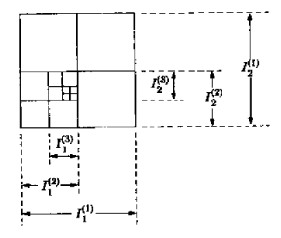
\includegraphics[scale=0.5]{img/I_2.png}
        \caption{\footnotesize{Imagen sacada del Apostol. Representación para cuando $\R^2$. Lo que queremos son todas las posibles combinaciones para $I_{1,k}^{(1)}$, $I_{2,k}^{(1)}$ (con $k=1$ y $k=2$). Es decir, todos los cuadrados posibles que se pueden formar al picar el cuadrado más grande por la mitad de forma vertical y horizontal (para $\R^2$ tenemos 4 posibles cuadrados).}}
        \label{fig:R^2}
    \end{marginfigure}
    
    Ahora, consideremos todos los productos de la forma
    
    \[
    I_{1,k_1}^{(1)} \times I_{2,k_1}^{(1)} \times \dots \times I_{n,k_n}^{(1)} \quad \text{con $k_i=1,2$}
    \]
    
    En total, existen $2^n$ productos de este tipo (por que hay dos posibles intervalos para cada $I_i$ con $i = 1, \dots, n$) y cada uno de ellos da como resultado un intervalo $n$-dimensional. Como la unión de estos $2^n$ intervalos es $J_1$ y $J_1$ contiene una cantidad infinita de puntos de $A$, entonces al menos un $J_2 = I_{j, k_j}^{(1)}$ que contiene una cantidad infinita de elementos de $A$. Este intervalo puede ser expresado como
    
    \[
    J_2 = \prod_{i=1} I_i^{(2)}
    \]
    
    \noindent donde cada $I_k^{(2)}$ es un subintervalo de $I_k^{(1)}$.
    
    Igual que antes, al bisecar cada uno de estos subintervalos, podemos encontrar un intervalo $n$-dimensional $J_3$ que contiene una cantidad infinita de puntos de $A$. Continuando este proceso, encontraremos una familia contable de intervalos $n$-dimensionales $J_1, J_2, J_3, \dots$ tales que el $m$-ésimo intervalo $J_m$ tiene infinitos puntos de $A$ y se puede expresar de la forma
    
    \[
    J_m = I_1^{(m)} \times I_2^{(m)} \times \dots \times I_n^{(m)} \quad \text{donde $I_k^{(m)} \subseteq I_k^{(1)}$}
    \]
    
    \noindent y además los $I_k^{(m)}$ son de la forma $I_k^{(m)} = [a_k^m, b_k^m]$. Y para cada uno de ellos su longitud es\marginfootnote{Recordemos que por cada "nivel" estamos bisecando los intervalos.}
    
    \[
    \left|b_k^{(m)} - a_k^{(m)}\right| = \frac{M}{2^{m-2}} \quad \text{donde $k = 1, \dots, n$}
    \]
    
    Observamos que la sucesión $\{a_k^{(m)}\}_{m=1}^{\infty}$ es creciente y al hacer $n \rightarrow \infty$, ella va a tender a $\sup_{m \geq 1} a_k$. Análogamente la sucesión $\{b_k^{(m)}\}_{m=1}^{\infty}$ es decreciente y al hacer $n \rightarrow \infty$, ella va a tender a $\inf_{m \geq 1} b_k^{(m)}$. Luego para cada $k$, estos valores coinciden en un valor en común $t_k$ al hacer $n \rightarrow \infty$.
    
    Sea $t = (t_1, t_2, \dots, t_n)$. Consideremos $B_2(t, r)$ para $r > 0$. Este punto $t$ está contenido en cada uno de los intervalos $J_1, J_2, \dots$ construídos anteriormente. Entonces cuando $m$ es tal que $M/2^{m-2} < r/2$ tneemos que la bola $B_2(t, r)$ contiene a $J_m$. Pero $J_m$ contiene una cantidad infinita de puntos de $A$ por construcción, entonces
    
    \[
    \left( B_2(t, r) \backslash \{t\} \right) \cap A \neq \emptyset
    \]
    
    Por lo tanto, $t$ es un punto de acumulación de $A$, y de esta forma queda demostrado.
\end{proof}

\begin{teo}[Cantor]
    Sea $(\Oc_j)_{j=1}^{\infty} \subset \R^n$ tal que
    
    \begin{itemize}
        \item $\Oc_{j+1} \subset \Oc_j$ para cada $j \geq 1$.
        \item $\Oc_j$ es cerrado, acotado y contiene infinitos elementos.
    \end{itemize}
    
    Entonces $\bigcap_j \Oc_j$ es cerrado y no-vacío.
\end{teo}

\begin{proof}
    Denotaremos por
    
    \[
    S = \bigcap_j \Oc_j
    \]
    
    Como $S$ es una intersección arbitraria de conjuntos cerrados, entonces es cerrado.
    
    Nos queda ver que $S$ es no-vacío. Como cada $\Oc_j$ es un conjunto con una cantidad infinita de elementos, entonces podemos definir
    
    \[
    A = \{x_1, x_2, \dots, x_j, \dots\} \quad \text{con $x_j \in \Oc_j$}
    \]
    
    Observamos que $A \subset \Oc_j$ ya que al tener $\Oc_{j+1} \subset \Oc_j$, entonces $x_1, \dots \in \Oc_1$. Como $\Oc_1$ es acotado, existe $M > 0$ tal que
    
    \[
    A \subset \Oc_1 \subset B(0, M)
    \]
    
    \noindent lo que implica que $A$ es acotado.
    
    Hemos verificado entonces que $A$ tiene infinitos elementos y $A$ es acotado. Entonces, por el teorema de Bolzano-Weierstrass, $A' \neq \emptyset$. Sea $a \in A'$, luego cada entorno de $a$ contiene una cantidad infinita de puntos de $A$ los cuales pertenecen a $\Oc_j$ (para cada $j$), salvo posiblemente una cantidad finita de ellos. Entonces este entorno también contiene una cantidad infinita de puntos de $\Oc_j$, por lo que $a \in \Oc_j'$. Pero como cada $\Oc_j$ es cerrado, entonces $a \in \Oc_j' = \Oc_j$ para todo $j$. Por lo tanto $a \in S$ y $S \neq \emptyset$.
    
    De esta manera queda demostrado.
\end{proof}

\subsection{Recubrimientos en $\R^n$}

\begin{defn}
    Una familia $\F = (A_j)_{j=1}^{\infty}$, tal que $A_j \subset \R^n$ y $A_j \neq \emptyset$ es un \ul{recubrimiento} de un conjunto $S \subset \R^n$ si $S \subset \bigcup_j A_j$.
    
    Si además, cada $A_j$ es abierto, decimos que el recubrimiento es por abiertos. Si cada $A_j$ es cerrado, decimos que el recubrimiento es por cerrados.
\end{defn}

\begin{teo}[Heine-Borel]
    Sea $\F$ un recubrimiento por abiertos de $A$, con $A$ cerrado y acotado en $\R^n$. Entonces hay una subcolección finita de $\F$ que cubren a $A$.
\end{teo}

\begin{proof}
    Denotemos a la familia de esta manera:
    
    \[
    \F = \left( I_j \right)_j \quad \text{tal que} \quad A \subset \bigcup_j I_j
    \]
    
    \noindent donde cada $I_j$ es abierto.
    
    Ahora definamos para cada $m \geq 1$ la unión
    
    \[
    S_m = \bigcup_{j=1}^m I_j
    \]
    
    Como cada $S_m$ es una unión arbitraria de abiertos, entonces $S_m$ es abierto. Por lo tanto $S_m^c = \R^n \backslash S_m$ es cerrado. Sean ahora $\{ \Oc_m \}_{m=1}^{\infty}$ tales que
    
    \[
    \Oc_1 = A, \qquad \Oc_m = A \cap S_m^c, \quad \text{si $m > 1$}
    \]
    
    Supongamos que $\Oc_m \neq \emptyset$ para todo $m$. Observemos que $\Oc_j = A \cap S_m^c$, y como $S_m$ crece, entonces $S_m^c$ decrece, por lo tanto $\{ \Oc_m \}_{m=1}^{\infty}$ decrece. Entonces tenemos que $\Oc_{m+1} \subset \Oc_m$ para todo $m$.
    
    Adicionalmente, también tenemos que
    
    \begin{itemize}
        \item Cada $\Oc_m$ es cerrado porque es la intersección de dos conjuntos cerrados.
        \item Cada $\Oc_m$ es acotado porque es la intersección de $S_m^c$ con el conjunto acotado $A$.
    \end{itemize}
    
    Entonces, por el teorema de Cantor, entonces $\bigcap_m \Oc_m \neq \emptyset$. Por lo tanto $\exists x_0$ tal que $x_0 \in A \wedge x_0 \in S_m^c$ para todo $m$. Esto implica que $x_0 \in A \wedge x_0 \notin S_m$ para todo $m$. Pero esto contradice el hecho de que $\F$ es un cubrimiento de $A$ ya que $A \subset_j I_j \subseteq \bigcup_k S_k$.
    
    Por lo tanto, existe algún $m_0$ para el cual $\Oc_{m_0} = \emptyset$. Lo cual implica que
    
    \[
    S_{m_0}^c \cap A = \emptyset \implies A \subset S_{m_0} = \bigcup_{j=1}^{m_0} I_j
    \]
    
    De esta forma, queda demostrado.
\end{proof}

\begin{defn}
    Un conjunto $A \subset \R^n$ es \ul{compacto} sii de todo cubrimiento por abiertos de $A$, podemos extraer un subcubrimiento finito.
\end{defn}

\begin{teo}
    Si $A \subset \R^n$ es compacto. Entonces $A$ es cerrado y acotado.
\end{teo}

\begin{proof}
    Sea $p \in A$ y consideremos la colección de $n$-bolas
    
    \[
    F = \{ B(p, k) \}_{k=1}^{\infty}
    \]
    
    \noindent donde $B(p, k) = \{ y \in \R^n : \normaeuc{y-p} < k \}$.
    
    Luego $A \subset \bigcup_{p \in A} \bigcup_{k=1}^{\infty} B(p, k)$. Pero $A$ es compacto, entonces existe al menos un $m_0 \in \N$ tal que
    
    \[
    A \subset \bigcup_{k=1}^{m_0} B(p, k)
    \]
    
    Como todas estas bolas son concéntricas, entonces
    
    \[
    A \subset \bigcup_{k=1}^{m_0} B(p, k) \subseteq B(p, m_0) \implies A \subset B(p, m_0)
    \]
    
    De esta forma, $A$ es un conjunto acotado, y queda verificar que $A$ es cerrado: Supongamos entonces que $A$ no es cerrado, entonces existe un elemento $y \in A'$ tal que $y \notin A$. Sea $x \in A$ y denotemos por $r_x = \normaeuc{x - y} / 2$. Luego la familia $\{ B_2(x, r_x) : x \in S \}$ es cubrimiento por abiertos de $A$. Pero $A$ es compacto, entonces hay una cantidad finita $n \in \N$ de estos entornos tales que la unión de ellos cubren a $A$, luego
    
    \[
    A \subset \bigcup_{k=1}^n B(x_k, r_{x_k})
    \]
    
    Consideremos $r = \min_{k=1, \dots, n} (r_k)$. Entonces
    
    \[
    B(y, r) \cap B(x_k, r_{x_k}) = \emptyset \quad \text{para todo $k=1, \dots, n$}
    \]
    
    En efecto es vacío, ya que si
    
    \[
    x \in B(y, r) \implies \normaeuc{x-y} < r \geq r_{x_k} \quad \text{para todo $k$}
    \]
    
    Y por la desigualdad triangular, tenemos que $\normaeuc{y-x_k} \leq \normaeuc{y-x} + \normaeuc{x - x_k}$. Luego
    
    \[
    \normaeuc{x - x_k} \geq \normaeuc{y-x_k} - \normaeuc{x-y} = 2r_k - \normaeuc{x-y} > r_k
    \]
    
    Y esto implica que $x \notin B_2(x_k, r_k)$. Entonces nos queda que
    
    \[
    B(y, r) \cap B(x_k, r_{x_k}) = \emptyset \quad \text{para todo $k=1, \dots, n$}
    \]
    
    Pero ya establecimos que $\bigcup_{k=1}^n B(x_k, r_{x_k})$ es un cubrimiento por abiertos de $A$. Entonces lo anterior implica que
    
    \[
    B(y, r) \cap A = \emptyset
    \]
    
    Luego $y$ no es punto de acumulación de $A$. Esto es una contradicción, ya que establecimos que $y \in A'$. Como estamos partiendo del hecho de suponer que $A$ no es cerrado, entonces necesariamente $A$ tiene que ser cerrado.
    
    De esta forma, queda demostrado que $A$ es cerrado y acotado.
\end{proof}
\section{Particiones de enteros}

\begin{defn}
    Dado un número entero no negativo $n$, denotamos por $p(n)$ a la cantidad de maneras de expresar $n$ como la suma de enteros positivos. Cada una de dichas maneras es una \ul{partición} de $n$ y si $\prop$ es una propiedad definida por un conjunto de restricciones para las particiones, denotamos por $p(n|\prop)$ a la cantidad de particiones de $n$ que tienen la propiedad $\prop$.
    
    Por ejemplo,
    
    \begin{gather*}
        p(5) = 7 \\
        p(10) = 42 \\
        p(100) = 190569292
    \end{gather*}
\end{defn}

Este concepto es bastante útil en por ejemplo esta clase de problemas:

\begin{prob}
    ¿De cuántas maneras se puede cambiar un billete de $100$ usando billetes de $50$, $20$, $10$ y $5$?:
    
    Esto equivale a contar la cantidad de maneras de expresar el número $100$ como suma de los números $50$, $20$, $10$ y $5$. En este caso, no es relevante el orden de los sumandos, cada sumando puede estar repetido e incluso es posble que uno o más de los números no se use. Es decir, se trata de contar las particiones del número 100, sujetas a la restricción debida a las denominaciones de los billetes a usar.
\end{prob}

\begin{notn}
    Dado un entero positivo $n$, es usual denotar por
    
    \[
    [1^{\alpha_1}2^{\alpha_2} \dots n^{\alpha_n}]
    \]
    
    \noindent a la partición de $n$ en la cual cada $i$ aparece $\alpha_i$ veces. Como es natural, si $\alpha_i=1$, se omite. Por ejemplo, si $n = 5$
    
    \begin{gather*}
        5 \leftrightarrow [5] \\
        4 + 1 \leftrightarrow [1 \ 4] \\
        2 + 2 + 1 \leftrightarrow [1 \ 2^2]
    \end{gather*}
    
    También es conveniente escribir las particiones de manera gráfica. Por ejemplo, la partición $[6 \ 5 \ 4^2 \ 2 \ 1^3]$ la graficamos así:
    
    \vspace{5mm}
    
    \begin{figure}
        \centering
        \begin{ferrers}
            \row{6} \row{5} \row{4} \row{4} \row{2} \row{1} \row{1} \row{1}
        \end{ferrers}
        \caption{Diagrama para la partición $[6 \ 5 \ 4^2 \ 2 \ 1^3]$.}
        \label{fig:ferrers1}
    \end{figure}
    
    Es decir, que para cada $i \leq n$ graficamos $\alpha_i$ filas, cada una con $i$ puntos. Esto se conoce como \textit{diagrama de Ferrers} para la partición.
\end{notn}

Estos diagramas son bastante convenientes en una cantidad diversa de problemas. Por ejemplo:

\begin{prob}
    Dados enteros positivos $n, r$, analicemos la partición
    
    \[
    p(n+r|\text{cantidad de partes $= r$})
    \]
    
    ¿Cómo es el diagrama de Ferrers para una partición de este tipo? ¿Cuántas marcas tiene la primera columna?
    
    \begin{marginfigure}
        \centering
        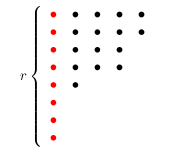
\includegraphics[scale=0.65]{img/ferrers2.png}
        \caption{Diagrama de Ferrers para la partición presentada en el problema. Vemos que la primera columna tiene $r$ puntos (uno para cada parte).}
        \label{fig:ferrers2}
    \end{marginfigure}
    
    Si se elimina la primera columna, queda el diagrama de una partición de $n$, y la partición que queda tiene a lo sumo $r$ partes. Es decir, a cada partición de $n+r$ con $r$ partes, le corresponde una partición de $n$ con a lo sumo $r$ partes.
    
    Ahora, dada una partición de $n$ con a lo sumo $r$ partes. ¿Podremos obtener una partición de $n+r$ con $r$ partes?: Basta con agregar una primera columna con $r$ puntos.
    
    \begin{marginfigure}
        \centering
        \begin{ferrers}
            \row{4} \row{4} \row{3} \row{3} \row{1}
        \end{ferrers}
        \caption{Acá estamos omitiendo la primera columna. Vemos que al agregarle la columna con $r$ puntos, estamos sumando $r$ puntos a la partición de $n$ que ya tenemos, por lo que resulta en $n+r$ puntos en total.}
    \end{marginfigure}
\end{prob}

Este hecho presentado en el problema puede resumirse de la siguiente manera.

\begin{teo}
    Dados enteros positivos $n$ y $r$,
    
    \[
    p(n+r|\text{cantidad de partes de $= r$}) = p(n|\text{cantidad de partes $\leq r$})
    \]
\end{teo}

Otro concepto que es útil para trabajar estos problemas es el de \textit{partición conjugada}. Dada una partición $\lambda$, la partición $\lambda'$ obtenida cambiando filas por columnas en el diagrama de Ferrers $\lambda$, se llama partición \textit{conjugada} de $\lambda$.

\begin{ejer}
    Dados enteros positivos $n$ y $m$, demuestra que la función dada por $\lambda \rightarrow \lambda'$ es una biyección entre el conjunto de las particiones de $n$ con parte máxima $m$ y el conjunto de las particiones de $n$ con $m$ partes. ¿Cómo se escribe esto con la notación $p(n|\prop)$?
\end{ejer}

\begin{proof}[Solución]
    La función $\lambda \rightarrow \lambda'$ es tal que las filas de $\lambda$ son las columnas de $\lambda'$. Entonces si $\lambda$ tiene $m$ partes, su primera columna tiene $m$ puntos, por lo tanto la primera fila de $\lambda'$ tiene $m$ puntos. De esta forma, la función $\lambda \rightarrow \lambda'$ es una biyección del conjunto de las partes de $n$ con parte máxima $m$ al conjunto de las partes de $n$ con $m$ partes. Luego
    
    \[
    p(n|\text{parte máxima = $m$}) = p(n|\text{$\#$ partes = $m$})
    \]
\end{proof}

Decimos que una partición $\lambda$ es \textit{autoconjugada} si $\lambda = \lambda'$. ¿Qué se puede decir de las particiones autoconjugadas a partir de su diagrama de Ferrers?

\begin{figure}
    \centering
    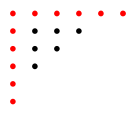
\includegraphics[scale=0.65]{img/ferrers3.png}
    \caption{Diagrama de Ferrers para la situación presentada.}
    \label{fig:ferrers3}
\end{figure}

Observemos el número total de puntos en la primera fila y primera columna. Si se eliminan esas marcas, ¿qué queda?: Como tienen la misma cantidad de puntos, digamos $k$, y como tienen un punto en común, el número total de puntos removidos es $2k-1$ (el cual es un número impar). De la misma forma, al remover las primera fila y columna en el nuevo diagrama, tendremos otra cantidad impar de puntos removidos, digamos $2l-1$. Haciendo esto de forma iterativa, encontraremos una nueva partición de $n$ donde cada una de sus partes es de tamaño impar y son todas distintas entre sí.

Equivalentemente, si tenemos una partición donde cada parte es de tamaño par y distintas entre sí, si cada parte es mayor que $1$ podemos formar una fila y una columna de tamaño, digamos $k+1$, tales que comparten un punto entre sí. Procediendo de manera iterativa, como cada una de las partes es distinta e impar, la partición resultante tendrá la característica de que al intercambiar las filas por columnas, cada una de ellas tendrá la misma cantidad de puntos en cada parte. De esta manera podemos enunciar el siguiente teorema:

\begin{teo}
    Dado un entero positivo $n$,
    
    \[
    p(n|\text{partes distintas e impares}) = p(n|autoconjugada)
    \]
\end{teo}

Sin embargo, calcular $p(n)$ no resulta algo tan trivial. Los métodos para encontrar $p(n)$ los encontraremos en las fórmulas generadoras y las sumas formales infinitas: Dados enteros positivos $n$ y $m$, analicemos

\[
a_n = p(n|\text{cada parte $= m$})
\]

Solamente podremos encontrar dichas particiones si $n$ es un múltiplo de $m$. Entonces $n$ es una partición $n = m + m + m + \dots$. Es decir,

\[
a_n =
\begin{cases}
    1 \quad \text{si $m$ divide a $n$} \\
    0 \quad \text{en otro caso}
\end{cases}
\]

Entonces definiendo $a_0 = 1$, tenemos

\[
\sumtoinfty{n=0}{a_nx^n} = 1 + x^m + x^{2m} + \dots
\]

Por lo tanto $f_m(x) = (1-x^m)^{-1}$ es una fórmula generadora para $p(n|\text{cada parte $= m$})$, con $n \geq 0$. Sea ahora un entero $r$ y definamos

\begin{gather*}
    b_n = p(n| \text{cada parte $=r$}) \\
    c_n = p(n| \text{cada parte $= m$ o $= r$})
\end{gather*}

¿Cómo podríamos calcular $c_n$? Observamos que $c_n$ es la cantidad de maneras de escribir $n$ como suma de $t$ y $n-t$ tales que $t$ está partido en partes de tamaño $m$ y $n-t$ está partido en partes de tamaño $r$. Entonces

\[
c_n = a_0b_n + a_1b_{n+1} + \dots + a_nb_0
\]

Y por definición de producto de sumas formales infinitas, la sucesión de los $c_n$ está generada por

\[
f_m(x)f_r(x) = (1-x^m)^{-1}(1-x^r)^{-1}
\]

De esta forma, podemos resolver problemas del siguiente tipo:

\begin{prob}
    ¿De cuántas maneras se puede escribir el número $10$ como sumas que sólo usan los números $2$ y $3$?: Basta con ver el coeficiente de $x^{10}$ en
    
    \[
    (1-x^2)^{-1}(1-x^3)^{-1}
    \]
    
    En cuyo caso obtenemos $2$.
\end{prob}

De forma análoga podemos concluir que para calcular $p(n|\text{cada parte $=i, j$ ó $k$})$ debemos hayar el coeficiente de $x^n$ en el producto 

\[
(1-x^i)^{-1}(1-x^j)^{-1}(1-x^k)^{-1}
\]

Usando esta idea podemos concluir que el coeficiente de $x^n$ en el producto

\[
(1-x^1)^{-1}(1-x^2)^{-1}\dots(1-x^n)^{-1}
\]

\noindent es la cantidad de particiones de $n$ en las que cada parte es de tamaño $1$, o $2$, \dots, o $n$. Es decir \textit{todas} las particiones de $n$. Conclusión: una fórmula generadora para $p(n)$ es

\[
P(x) = \prod_{i=1}^{\infty} (1-x^i)^{-1}
\]

\subsection{Calcularndo $p(n)$}

Los métodos expuestos anteriormente nos permiten escribir funciones generadoras para los números de particiones tales que se satisfacen ciertas restricciones: ¿Qué ocurre si cada parte aparece a lo sumo $k$ veces? En ese caso tendremos un factor de la forma

\[
(1 + x^i + x^{2i} + \dots + x^{ki}), \quad \text{para cada tamaño $i$}
\]

\noindent en lugar de la suma formal infinita. En consecuencia una fórmula generadora sería

\[
\prod_{i=1}^{\infty} (1 + x^i + x^{2i} + \dots + x^{ki}) = \prod_{i=1}^{\infty} \frac{1 - x^{(k+1)i}}{1-x^i}
\]

En particular, si tenemos $k=1$ entonces esto nos da

\[
p(n | \text{partes son distintas}) = (1+x)(1+x^2)(1+x^3)\dots
\]

Otras fórmulas generadoras sencillas (y fácilmente verificables) son

\begin{gather*}
    p(n | \text{partes con tamaño impar}) = \frac{1}{(1-x)(1-x^3)(1-x^5)\dots} \\
    p(n | \text{partes con tamaño par}) = \frac{1}{(1-x^2)(1-x^4)(1-x^6)\dots} \\
    p(n | \text{partes con tamaño $\leq m$}) = \frac{1}{(1-x)(1-x^2)\dots(1-x^m)}
\end{gather*}

Observemos que a partir de

\[
(1+x)(1+x^2)(1+x^3)\dots
\]

\noindent al multiplicar y dividir por $(1-x^i)$ con $i = 1, 2, \dots$ nos queda que

\[
\frac{(1-x^2)(1-x^4)(1-x^6) \dots}{(1-x)(1-x^2)(1-x^3) \dots}  = \frac{1}{(1-x)(1-x^3)(1-x^5) \dots}
\]

En conclusión, para cada $n$, $p(n | \text{partes con tamaño impar})$ y $p(n | \text{partes dinstintas})$ tienen la misma fórmula generadora, por lo que

\[
p(n | \text{partes con tamaño impar}) = p(n | \text{partes distintas})
\]

Ahora, recordemos que la fórmula

\[
P(x) = \prod_{i=1}^{\infty}(1-x^i)^{-1}
\]

\noindent genera la suceción $\{p(n)\}_{n=0}^{\infty}$. Si multiplicamos esto por

\[
Q(x) = \prod_{i=1}^{\infty} (1-x^i)
\]

\noindent el resultado es 1, entonces el coeficiente de $x^n$ en $P(x)Q(x)$ para $n \geq 1$ es cero, por lo que se cumple

\[
q_0P(n) + q_1P(n-1) + \dots + q_n = 0
\]

Es decir, que si conocemos los $q_n$'s podremos obtener una relación recursiva para $p(n)$, así que analicemos $Q(x)$. Calculando los primeros términos se obtiene

\[
1 - x - x^2 + x^5 + x^7 - x^{12} - x^{15} + x^{22} + x^{26} - \dots
\]

Aparentemente la mayoría de los coeficientes son cero, mientras que el resto es $1$ ó $-1$. Para ver esto claramente, primero recordemos el producto

\[
p(n | \text{partes son distintas}) = (1+x)(1+x^2)(1+x^3)\dots
\]

En este caso, la partición $7 = 1 + 2 + 4$ corresponde al término $x \times x^2 \times x^4$ y suma $1$ al coeficiente de $x^7$. Consideremos ahora el mismo producto, pero cambiando los signos. Entonces tendremos

\[
Q(x) = \prod_{i=1}^{\infty} (1-x^i) = (1-x)(1-x^2)(1-x^3)\dots
\]

En este caso, la partición $7 = 1 + 2 + 4$ corresponde al término $(-x) \times (-x)^2 \times (-x)^4$ y suma $-1$ al coeficiente de $x^7$. Por lo tanto cada partición de $n$ con partes distintas suma $(-1)^d$ al coeficiente de $x^n$, donde $d$ es la cantidad de partes. Y en general, cada partición de $n$ con una cantidad par de partes distintas suma $1$ a $q_n$, y cada partición de $n$ con una cantidad impar de partes distintas suma $-1$ a $q_n$. Por lo tanto si denotamos por

\begin{gather*}
    e_n = p(n | \text{partes distintas y $\#$ partes par}) \\
    o_n = p(n | \text{partes distintas y $\#$ partes impar})
\end{gather*}

Entonces $q_n = e_n - o_n$. Por lo tanto $q_n = 0$ si $e_n = o_n$.

Analicemos los casos en que $q_n \neq 0$: Para cada partición $\lambda$ con partes distintas, definamos una partición $\lambda'$ tal que la correspondencia será biyectiva en la mayoría de los casos, y para el resto la biyectividad fallará. Denotemos también por $s(\lambda)$ a la parte más pequeña de $\lambda$, y si $\lambda$ tiene $m$ partes, enumeraremos las filas en su diagrama de Ferrers de arriba hacia abajo. Si para cada $i < m$ la fila $i$ tiene exactamente un punto más que la fila $i+1$, definimos $t(\lambda) = m$; en caso contrario, $t(\lambda)$ es el mínimo $i$ tal que la fila $i$ \textbf{no} tiene exactamente un punto más que la fila $i+1$.

\begin{figure}
    \centering
    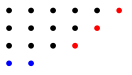
\includegraphics[scale=0.65]{img/ferrers4.png}
    \caption{En este ejemplo, $s(\lambda) = 2$ y $t(\lambda) = 3$.}
    \label{fig:ferrers4}
\end{figure}

Para definir la correspondencia $\lambda \rightarrow \lambda'$ consideraremos dos casos. Si $s(\lambda) \leq t(\lambda)$, eliminamos la parte $s(\lambda)$ y cada punto eliminado lo colocaremos al final de cada una de las $s(\lambda)$ filas del diagrama.

\begin{figure}
    \centering
    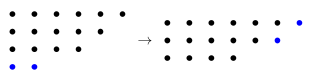
\includegraphics[scale=0.65]{img/ferrers5.png}
    \caption{Vemos aquí que los puntos azules de $\lambda$ se colocan al final de las 2 primeras filas de $\lambda'$.}
    \label{fig:ferrers5}
\end{figure}

Si $s(\lambda) > t(\lambda)$ eliminamos el último punto de cada una de las primeras $t(\lambda)$ y con ellos formamos una nueva última fila.

\begin{figure}
    \centering
    
\includegraphics[scale=0.65]{img/ferrers6.png}
    \caption{Los puntos rojos de $\lambda'$ se corresponden con los últimos puntos de las primeras $t(\lambda)$ filas de $\lambda$.}
    \label{fig:ferrers6}
\end{figure}

Resaltamos que la cantidad de partes de $\lambda$ y $\lambda'$ difieren en $1$, por lo que a una partición contada por $e_n$, le corresponde una partición contada por $o_n$ y viceversa. Esta es \textbf{casi} una correspondencia biyectiva, pero ¿cuáles son las excepciones? En el primer caso, si $s(\lambda) = t(\lambda)$ y los puntos correspondientes se solapan, la operación \textbf{no} produce el diagrama de una partición.

\begin{figure}
    \centering
    
\includegraphics[scale=0.65]{img/ferrers7.png}
    \caption{Vemos que los puntos se solapan.}
    \label{fig:ferrers7}
\end{figure}

Para este caso, $s(\lambda) = m$ y

\[
n = m + (m+1) + (m+1) + \dots + (m+m-1) = \frac{m(3m-1)}{2}
\]

En el segundo caso, si los puntos correspondientes se solapan y $s(\lambda) = m+1$, entonces $\lambda'$ tiene las últimas dos partes iguales.

\begin{figure}
    \centering
    
\includegraphics[scale=0.65]{img/ferrers8.png}
    \caption{Vemos nuevamente que los puntos se solapan y $\lambda \rightarrow \lambda'$ no es biyectiva en este caso.}
    \label{fig:ferrers8}
\end{figure}

En este caso tenemos que

\[
n = m + (m+1) + (m+1) + \dots + (m+m) = \frac{m(3m+1)}{2}
\]

Estos resultados los podemos resumir de la siguiente manera:

\begin{teo}
    Si $Q(x)$ está definida por
    
    \[
    Q(x) = \sum_{n=0}^{\infty} q_nx^n = (1-x)(1-x^2)\dots
    \]
    
    \noindent entonces
    
    \[
    q_n = \begin{cases}
              (-1)^m \quad &\text{si $\displaystyle n = \frac{m(3m \pm 1)}{2}$} \\
              0 \quad &\text{en otro caso}
          \end{cases}
    \]
\end{teo}

De esta forma, se obtienen algunos valores no nulos de $q_n$:

\begin{center}
    \begin{tabular}{ccc}
        $m$ & $\displaystyle \frac{m(3m-1)}{2}$ & $\displaystyle \frac{m(3m+1)}{2}$ \\ \toprule
        $1$ & $1$ & $2$ \\
        $2$ & $5$ & $7$ \\
        $3$ & $12$ & $15$ \\
        $4$ & $22$ & $26$ \\
        $5$ & $35$ & $40$ \\
        $6$ & $51$ & $57$
    \end{tabular}
\end{center}

Con lo cual se puede obtener la recurrencia para $p(n)$:

\[
p(n) = p(n-1) + p(n-2) - p(n-5) - p(n-7) + p(n-12) + p(n-15) + \dots
\]

\end{document}